% ============================================================
% GRADUATION THESIS
% Network Quality of Service (QoS) Scheduling System
% on the Android Platform
% ============================================================
% Compiler: XeLaTeX (Unicode support)
% ============================================================

\documentclass[a4paper, 11pt, oneside]{report}

% ======================== PACKAGES ========================

% --- Font & Language support ---
\usepackage{fontspec}
\setmainfont{Times New Roman}
\usepackage{polyglossia}
\setdefaultlanguage{english}

% --- Page layout ---
\usepackage[
    top=3.5cm,
    bottom=3cm,
    left=3.5cm,
    right=2cm,
    headheight=15pt
]{geometry}

% --- Typography & Spacing ---
\usepackage{setspace}
\setstretch{1.2}
\setlength{\parindent}{1.27cm}
\setlength{\parskip}{6pt}

% --- Headers & Footers ---
\usepackage{fancyhdr}
\pagestyle{fancy}
\fancyhf{}
\fancyhead[R]{\small\nouppercase{\leftmark}}
\fancyfoot[C]{\thepage}
\renewcommand{\headrulewidth}{0.4pt}
\renewcommand{\footrulewidth}{0pt}

% --- Chapter & Section styling ---
\usepackage{titlesec}

\titleformat{\chapter}[display]
{\normalfont\LARGE\bfseries\centering}
{\MakeUppercase{\chaptertitlename}\ \thechapter}{20pt}{\LARGE\MakeUppercase}
\titlespacing*{\chapter}{0pt}{-20pt}{30pt}

\titleformat{\section}
{\normalfont\large\bfseries}{\thesection}{1em}{}
\titleformat{\subsection}
{\normalfont\normalsize\bfseries}{\thesubsection}{1em}{}
\titleformat{\subsubsection}
{\normalfont\normalsize\itshape}{\thesubsubsection}{1em}{}

% --- Table of Contents depth ---
\setcounter{tocdepth}{3}
\setcounter{secnumdepth}{3}

% --- Graphics ---
\usepackage{graphicx}
\usepackage{float}
\graphicspath{{images/}}

% --- Tables ---
\usepackage{booktabs}
\usepackage{array}
\usepackage{longtable}
\usepackage{multirow}
\usepackage{tabularx}

% --- Code listings ---
\usepackage{listings}
\usepackage{xcolor}

\definecolor{codegreen}{rgb}{0,0.6,0}
\definecolor{codegray}{rgb}{0.5,0.5,0.5}
\definecolor{codepurple}{rgb}{0.58,0,0.82}
\definecolor{backcolour}{rgb}{0.97,0.97,0.97}
\definecolor{framecolor}{rgb}{0.8,0.8,0.8}

\lstdefinestyle{kotlinstyle}{
    backgroundcolor=\color{backcolour},
    commentstyle=\color{codegreen}\itshape,
    keywordstyle=\color{blue}\bfseries,
    numberstyle=\tiny\color{codegray},
    stringstyle=\color{codepurple},
    basicstyle=\ttfamily\small,
    breakatwhitespace=false,
    breaklines=true,
    captionpos=b,
    keepspaces=true,
    numbers=left,
    numbersep=8pt,
    showspaces=false,
    showstringspaces=false,
    showtabs=false,
    tabsize=4,
    frame=single,
    rulecolor=\color{framecolor},
    xleftmargin=15pt,
    framexleftmargin=15pt,
}

\lstset{style=kotlinstyle}

% --- Math ---
\usepackage{amsmath}
\usepackage{amssymb}

% --- Algorithms ---
\usepackage{algorithm}
\usepackage{algpseudocode}

% --- Hyperlinks ---
\usepackage[
    colorlinks=true,
    linkcolor=black,
    citecolor=blue,
    urlcolor=blue,
    bookmarks=true,
    bookmarksnumbered=true
]{hyperref}

% --- Bibliography ---
\usepackage[numbers,sort&compress]{natbib}

% --- Captions ---
\usepackage{caption}
\captionsetup{
    font=small,
    labelfont=bf,
    format=hang,
    justification=centering
}

% --- Misc ---
\usepackage{enumitem}
\usepackage{pdfpages}

% ======================== CUSTOM COMMANDS ========================

\newcommand{\qosapp}{\textit{QoS Scheduler}}
\newcommand{\android}{\textit{Android}}
\newcommand{\TODO}[1]{\textcolor{red}{\textbf{[TODO: #1]}}}

% ======================== DOCUMENT ========================

\begin{document}

% ---- Front Matter ----
\pagenumbering{roman}

% --- Title Page ---
% ============================================================
% TITLE PAGE
% ============================================================

\begin{titlepage}
\begin{center}

% --- Header ---
\textbf{\large MINISTRY OF EDUCATION AND TRAINING}\\[3pt]
\textbf{\large UNIVERSITY OF SCIENCE AND TECHNOLOGY OF HANOI}\\[3pt]
\textbf{\large FACULTY OF ICT DEPARTMENT}\\[5pt]

\rule{\textwidth}{1.5pt}\\[1cm]

% --- Logo ---
% 
\includegraphics[width=3cm]{logo.png}\\[1cm]
\vspace{1cm}

% --- Title ---
{\Large \textbf{GRADUATION THESIS}}\\[0.5cm]
{\large Major: Information and Communication Technology}\\[1.5cm]

{\LARGE \textbf{A NETWORK QUALITY OF SERVICE (QoS)}}\\[0.3cm]
{\LARGE \textbf{SCHEDULING SYSTEM}}\\[0.3cm]
{\LARGE \textbf{ON THE ANDROID PLATFORM}}\\[2cm]

% --- Author info ---
\begin{tabular}{rl}
\textbf{Student:} & Pham Hieu Minh \\[5pt]
\textbf{Student ID:} & 23BI14295 \\[5pt]
\textbf{Class:} & ICT \\[5pt]
\textbf{Supervisor:} & Le Huy Quang \\[5pt]
\end{tabular}

\vfill

% --- Footer ---
\rule{\textwidth}{1.5pt}\\[10pt]
{\large \textbf{Ha Noi, June 2026}}

\end{center}
\end{titlepage}


% --- Declaration ---
% ============================================================
% DECLARATION OF ORIGINALITY
% ============================================================

\chapter*{DECLARATION OF ORIGINALITY}
\addcontentsline{toc}{chapter}{Declaration of Originality}

I hereby declare that this thesis is the result of my own original research, conducted under the academic supervision of \TODO{Supervisor Name}.

All data, experimental results, and findings presented in this thesis are truthful and have not been previously published in any other work. All referenced materials have been fully and properly cited.

I accept full responsibility for the content and integrity of this thesis.

\vspace{2cm}

\begin{flushright}
\textit{Ho Chi Minh City, \TODO{Day} \TODO{Month} 2026}\\[1.5cm]
\textbf{Student}\\[1.5cm]
\TODO{Full Name}
\end{flushright}


% --- Acknowledgements ---
% ============================================================
% ACKNOWLEDGEMENTS
% ============================================================

\chapter*{ACKNOWLEDGEMENTS}
\addcontentsline{toc}{chapter}{Acknowledgements}

First and foremost, I would like to express my sincere and deepest gratitude to \TODO{Supervisor Name}, who directly guided, patiently mentored, and provided invaluable direction throughout the entire process of completing this graduation thesis.

I would also like to thank the faculty members of the \TODO{Faculty Name}, \TODO{University Name}, for imparting valuable knowledge throughout my academic journey, which formed the solid foundation that enabled me to complete this thesis.

Finally, I wish to extend my heartfelt thanks to my family and friends, who have continuously encouraged and supported me during this time.

Despite my best efforts, due to limitations in knowledge and time, this thesis may contain certain shortcomings. I sincerely welcome any constructive feedback from the faculty and peers to further improve this work.

\vspace{1.5cm}

\begin{flushright}
\textit{Ho Chi Minh City, \TODO{Month} 2026}\\[1cm]
\textbf{Student}\\[1.2cm]
\TODO{Full Name}
\end{flushright}


% --- Abstract ---
% ============================================================
% ABSTRACT
% ============================================================

\chapter*{ABSTRACT}
\addcontentsline{toc}{chapter}{Abstract}

As the number of mobile applications continues to grow and network usage demands diversify, controlling Quality of Service (QoS) on mobile devices has become a critical technical challenge. Existing solutions on Android either require Root privileges --- impractical for most users --- or only provide basic firewall functionality without priority-based bandwidth scheduling capabilities.

This thesis presents the design and implementation of \textbf{QoS Scheduler} --- an Android application capable of intervening at the network layer (Layer 3) to perform per-application bandwidth scheduling \textbf{without requiring Root access}. The system utilizes the TUN virtual network interface through the Android VpnService API to intercept, analyze, and schedule all IP traffic on the device.

The main contributions of this thesis include:
\begin{itemize}
    \item A Data Plane module capable of bit-level IPv4/IPv6 and TCP/UDP header parsing, including IPv6 Extension Header Chaining support.
    \item Implementation of the \textbf{Token Bucket} algorithm for rate limiting and \textbf{Weighted Fair Queuing (WFQ)} for priority-weighted bandwidth allocation (HIGH/MEDIUM/LOW).
    \item A UID Resolution mechanism based on 5-tuple information for per-application traffic classification.
    \item A stable TCP/UDP Relay system compatible with multiple Android versions, including custom ROMs such as HyperOS/MIUI.
\end{itemize}

Experimental results demonstrate the system's ability to accurately limit bandwidth, allocate network resources by weight with less than 5\% deviation, and mitigate Bufferbloat for high-priority applications.

\vspace{1cm}
\noindent\textbf{Keywords:} Quality of Service, QoS, Android, VPN, Token Bucket, Weighted Fair Queuing, Packet Analysis, Bandwidth Scheduling.


% --- Table of Contents ---
\tableofcontents
\newpage

% --- List of Figures ---
\listoffigures
\addcontentsline{toc}{chapter}{List of Figures}
\newpage

% --- List of Tables ---
\listoftables
\addcontentsline{toc}{chapter}{List of Tables}
\newpage

% --- Glossary ---
% ============================================================
% LIST OF ABBREVIATIONS
% ============================================================

\chapter*{LIST OF ABBREVIATIONS}
\addcontentsline{toc}{chapter}{List of Abbreviations}

\begin{longtable}{@{}p{3cm}p{10cm}@{}}
\toprule
\textbf{Abbreviation} & \textbf{Description} \\
\midrule
\endhead

ACK     & Acknowledgement \\
API     & Application Programming Interface \\
DPI     & Deep Packet Inspection \\
DSCP    & Differentiated Services Code Point \\
DNS     & Domain Name System \\
FIN     & Finish (TCP connection termination flag) \\
HTTP    & HyperText Transfer Protocol \\
HTTPS   & HTTP Secure \\
IETF    & Internet Engineering Task Force \\
IHL     & Internet Header Length \\
IP      & Internet Protocol \\
IPv4    & Internet Protocol version 4 \\
IPv6    & Internet Protocol version 6 \\
ISN     & Initial Sequence Number \\
JSON    & JavaScript Object Notation \\
MTU     & Maximum Transmission Unit \\
MVVM    & Model-View-ViewModel \\
OS      & Operating System \\
OSI     & Open Systems Interconnection \\
QoS     & Quality of Service \\
RFC     & Request for Comments \\
RST     & Reset (TCP connection reset flag) \\
RTT     & Round-Trip Time \\
SDK     & Software Development Kit \\
SYN     & Synchronize (TCP synchronization flag) \\
TCP     & Transmission Control Protocol \\
TTL     & Time to Live \\
TUN     & Network Tunnel (virtual network interface) \\
UDP     & User Datagram Protocol \\
UI      & User Interface \\
UID     & User Identifier (Android application identifier) \\
VoIP    & Voice over Internet Protocol \\
VPN     & Virtual Private Network \\
WFQ     & Weighted Fair Queuing \\

\bottomrule
\end{longtable}

\newpage

% ---- Main Matter ----
\pagenumbering{arabic}

% ============================================================
% CHAPTER 1: INTRODUCTION
% ============================================================

\chapter{INTRODUCTION}
\label{chap:introduction}

\section{Problem Statement and Motivation}
\label{sec:problem_statement}

Over the past decade, smartphones have become the primary Internet-connected devices for billions of users worldwide. According to the Ericsson Mobility Report 2024, global mobile data traffic has reached an average of 17 GB per user per month and is projected to triple by 2029 \cite{ericsson2024}. This surge is driven by the proliferation of bandwidth-intensive applications such as video streaming (YouTube, Netflix), video conferencing (Zoom, Google Meet), online gaming (Mobile Legends, PUBG Mobile), and social media (TikTok, Facebook).

Each of the aforementioned applications has distinct network Quality of Service (QoS) requirements. Online gaming demands ultra-low latency --- below 50 milliseconds --- with stable jitter. Video streaming requires sustained bandwidth at 5--8 Mbps for HD quality. Meanwhile, background activities such as downloading updates or cloud synchronization can tolerate lower speeds without degrading the user experience.

However, the Android operating system --- commanding over 72\% of the global mobile market share according to StatCounter (2024) \cite{statcounter2024} --- does not provide per-application bandwidth scheduling mechanisms for ordinary users. Android's network stack employs a default ``best-effort'' policy: all applications receive equal treatment in terms of network resource access. This leads to a common scenario: when a single application consumes the entire available bandwidth through a large download, latency-sensitive applications (such as games or video calls) suffer severe performance degradation --- a phenomenon known as \textit{Bufferbloat} \cite{gettys2012bufferbloat}.

Existing solutions on Android can be categorized into two main groups. The first group consists of applications that require Root access (e.g., AFWall+ \cite{afwall}, NetHogs \cite{nethogs}), which allow direct manipulation of iptables within the Linux kernel but are impractical for the vast majority of users due to warranty violations and potential security risks. The second group comprises non-Root firewall applications (e.g., NetGuard \cite{netguard}, GlassWire \cite{glasswire}), which utilize the VpnService API but only provide allow/deny functionality \textbf{without the ability to schedule bandwidth according to priority levels}.

This technical gap is the primary motivation for this thesis: to build a system capable of \textbf{intervening at the network layer (Layer 3) to perform per-application QoS scheduling without requiring Root access} on Android devices.

% -----------------------------------------------------------

\section{Research Evolution: From Hotspot QoS to Per-Application QoS}
\label{sec:research_evolution}

It is important to document that the scope of this thesis underwent a significant and deliberate evolution during the early research phase. The \textbf{original research goal} was to build a QoS scheduling system for \textit{devices connected to the host phone's WiFi Hotspot} --- i.e., per-device bandwidth management in a mobile hotspot environment. The envisioned scenario was a user sharing their mobile data via WiFi Hotspot (e.g., in a dormitory, small office, or public setting) and wanting to control how much bandwidth each connected device could consume.

However, a thorough feasibility analysis during the preliminary research phase revealed that \textbf{per-device hotspot QoS is technically infeasible on unrooted Android devices}, due to the following fundamental platform limitations:

\begin{enumerate}
    \item \textbf{VPN tunnel does not capture hotspot traffic:} The Android VpnService API creates a TUN interface that intercepts traffic originating from the \textit{host device's own network stack}. Traffic forwarded between the hotspot interface (\texttt{ap0} or \texttt{swlan0}) and the upstream WAN interface is handled by the Linux kernel's IP forwarding subsystem (\texttt{netfilter/iptables}). This forwarded traffic \textbf{does not pass through the TUN interface} on most Android versions and devices, making it invisible to a VpnService-based application.

    \item \textbf{No per-application visibility on connected devices:} Even on Android versions where hotspot traffic does traverse the VPN tunnel, the host device can only observe the \textit{source IP address} of the connected device (e.g., \texttt{192.168.43.x}). It has \textbf{no mechanism to identify which application} on the connected device generated the traffic, since the \texttt{ConnectivityManager.getConnectionOwnerUid()} API only resolves UIDs for locally-owned connections.

    \item \textbf{Device identification requires Root:} Reliable identification of connected devices via MAC address requires reading the kernel's ARP table (\texttt{/proc/net/arp}), which is accessible without Root but produces unreliable results on newer Android versions due to MAC address randomization. Furthermore, associating traffic flows with specific client devices across NAT boundaries requires kernel-level hooks unavailable in userspace.

    \item \textbf{Inconsistent behavior across ROMs and versions:} Testing revealed that hotspot traffic routing through VPN varies significantly across Android versions (10--14), manufacturers (Samsung, Xiaomi, Google), and custom ROMs (MIUI, OneUI). This inconsistency makes it impossible to build a reliable, universal solution.
\end{enumerate}

Based on this analysis, the research scope was \textbf{pivoted} from per-device hotspot QoS to \textbf{per-application QoS on the host device itself}. This pivot was a deliberate engineering decision driven by the following reasoning:

\begin{itemize}
    \item \textbf{Broader applicability:} Per-application QoS benefits \textit{every} Android user --- not just those who share their connection via Hotspot. Any user running multiple applications simultaneously (e.g., gaming while a background app downloads updates) can benefit from bandwidth prioritization.
    
    \item \textbf{Technical soundness:} The VpnService API provides complete and reliable access to all traffic from the host device's own applications, making per-application QoS technically robust and universally compatible across all Android 10+ devices.
    
    \item \textbf{Foundation for future extension:} The core QoS engine (Token Bucket, WFQ, packet parsing) built for per-application scheduling forms the architectural foundation upon which per-device hotspot QoS can be added in the future --- potentially on rooted devices or when Android introduces new APIs for hotspot traffic interception.
\end{itemize}

The remnants of the original hotspot vision are preserved in the codebase through the \texttt{HotspotManager} (hotspot detection and subnet identification) and \texttt{DeviceRegistry} (connected device tracking) modules, which remain functional and are documented in Chapter~5. These modules demonstrate the research effort invested in the original direction and provide a starting point for the hotspot QoS extension described in Chapter~7.

% -----------------------------------------------------------

\section{Research Objectives}
\label{sec:research_objectives}

This thesis establishes the following specific research objectives:

\subsection{General Objective}
To design and implement an Android application capable of scheduling network Quality of Service (QoS) on a per-application basis, operating at the network layer (Layer 3) through a virtual TUN interface without requiring Root privileges.

\subsection{Specific Objectives}

\begin{enumerate}[label=\textbf{SO\arabic*.}]
    \item \textbf{Packet Interception and Analysis:} Build a module capable of intercepting 100\% of IP traffic traversing the device and accurately parsing IPv4, IPv6, TCP, and UDP header structures at the bit level using bitwise operations.
    
    \item \textbf{Application Identification:} Develop a mechanism to identify the application owning each network flow based on Android's UID (User Identifier), using 5-tuple information (Protocol, Source IP, Source Port, Destination IP, Destination Port).
    
    \item \textbf{Bandwidth Scheduling:} Implement the Token Bucket algorithm for rate limiting and Weighted Fair Queuing (WFQ) for priority-weighted bandwidth allocation across applications.
    
    \item \textbf{Data Relay:} Build a TCP and UDP Proxy/Relay system that transparently forwards data to the real Internet, invisible to the applications running on the device.
    
    \item \textbf{Experimental Validation:} Evaluate the system's effectiveness through testing scenarios using iPerf3, Wireshark, and internal diagnostic logging.
\end{enumerate}

% -----------------------------------------------------------

\section{Research Scope}
\label{sec:research_scope}

\subsection{Research Subjects}
\begin{itemize}
    \item The networking management mechanisms of the Android operating system, specifically the VpnService API and the virtual TUN network interface.
    \item IP packet structures (IPv4/IPv6), TCP and UDP as defined by their respective RFC standards.
    \item Bandwidth scheduling algorithms: Token Bucket and Weighted Fair Queuing.
    \item Network traffic classification techniques based on destination port and application UID.
\end{itemize}

\subsection{Scope Boundaries}
\begin{itemize}
    \item \textbf{Platform:} Android 10 (API Level 29) and above --- the minimum version supporting the \texttt{ConnectivityManager.getConnectionOwnerUid()} API.
    \item \textbf{Network Layers:} Layer 3 (Network Layer) and Layer 4 (Transport Layer) of the OSI model.
    \item \textbf{Protocols:} IPv4, IPv6, TCP, UDP.
    \item \textbf{Programming Language:} Kotlin.
    \item \textbf{Limitation:} This thesis focuses on outbound traffic from the device. Inbound traffic is handled indirectly through TCP's congestion feedback mechanism.
\end{itemize}

% -----------------------------------------------------------

\section{Research Methodology}
\label{sec:research_methodology}

This thesis employs a combination of two primary research methods:

\subsection{Theoretical Research}
\begin{itemize}
    \item Study of Internet standards (RFCs) related to IPv4 (RFC 791) \cite{rfc791}, IPv6 (RFC 8200) \cite{rfc8200}, TCP (RFC 9293) \cite{rfc9293}, UDP (RFC 768) \cite{rfc768}, and the Checksum computation algorithm (RFC 1071) \cite{rfc1071}.
    \item Analysis of the Android operating system architecture and APIs, specifically VpnService \cite{android_vpnservice}, ConnectivityManager \cite{android_connectivity}, and the Socket Protection mechanism.
    \item Comparative analysis of QoS scheduling algorithms: Token Bucket, Leaky Bucket, Weighted Fair Queuing, and Deficit Round Robin.
\end{itemize}

\subsection{Experimental Research}
The experimental methodology applies a \textbf{``Triple-Lock Verification''} approach --- collecting data simultaneously from three independent sources to ensure objectivity:

\begin{enumerate}
    \item \textbf{Internal Application Logs} (Internal Diagnostic Logging): Recording QoS algorithm operational metrics within the application (actual throughput in Mbps, packet drop rate, number of processed packets).
    
    \item \textbf{End-to-End Measurement:} Using the iPerf3 tool \cite{iperf3} to measure throughput, latency, jitter, and packet loss from the end-user perspective.
    
    \item \textbf{Packet-level Analysis:} Using Wireshark \cite{wireshark} to capture and analyze packets at the protocol level, verifying changes in TCP Window Size, RTT, and retransmission rate when the QoS system is active.
\end{enumerate}

% -----------------------------------------------------------

\section{Scientific and Practical Significance}
\label{sec:significance}

\subsection{Scientific Significance}
\begin{itemize}
    \item Demonstrates the feasibility of implementing enterprise-grade QoS algorithms (Token Bucket, WFQ) on Android mobile devices without kernel-level intervention (no Root access required).
    \item Proposes the ``Triple-Lock Verification'' methodology for validating QoS system effectiveness on mobile platforms --- a methodology applicable to future similar research.
    \item Analyzes and resolves Android-specific technical challenges: the Routing Loop problem, custom ROM compatibility (MIUI), and the Socket Protection mechanism throughout the VPN lifecycle.
\end{itemize}

\subsection{Practical Significance}
\begin{itemize}
    \item Provides a solution for ordinary Android users to control bandwidth allocation among applications: prioritizing games and video calls while throttling background downloads.
    \item The application can be deployed in real-world scenarios: WiFi Hotspot sharing in cafes, dormitories, or small offices where bandwidth control across multiple devices is needed.
    \item The open-source codebase allows the developer community to continue extending and improving the system.
\end{itemize}

% -----------------------------------------------------------

\section{Thesis Organization}
\label{sec:organization}

This thesis is organized into seven chapters as follows:

\begin{itemize}[leftmargin=2cm]
    \item[\textbf{Chapter 1:}] \textbf{Introduction} --- Presents the problem statement, research objectives, scope, methodology, and significance of the thesis.
    
    \item[\textbf{Chapter 2:}] \textbf{Related Work} --- Surveys and analyzes existing QoS solutions on Android, related research, and positions this thesis within the broader research landscape.
    
    \item[\textbf{Chapter 3:}] \textbf{Theoretical Foundation} --- Presents the theoretical background on IP, TCP, and UDP protocols, QoS algorithms (Token Bucket, WFQ), and VPN technology on Android.
    
    \item[\textbf{Chapter 4:}] \textbf{System Analysis and Design} --- Analyzes requirements, designs the system architecture following the Data Plane/Control Plane model, and provides detailed module specifications.
    
    \item[\textbf{Chapter 5:}] \textbf{Implementation} --- Presents the detailed implementation process, low-level programming techniques, and technical challenges that were resolved.
    
    \item[\textbf{Chapter 6:}] \textbf{Testing and Evaluation} --- Presents the testing methodology, experimental results, data analysis, and system effectiveness evaluation.
    
    \item[\textbf{Chapter 7:}] \textbf{Conclusion and Future Work} --- Summarizes the achieved results, identifies limitations, and proposes future development directions.
\end{itemize}

\noindent In addition, the thesis includes \textbf{References} and \textbf{Appendices} containing source code of key modules, detailed test results, and the application user manual.

% ============================================================
% CHAPTER 2: LITERATURE REVIEW AND THEORETICAL BACKGROUND
% ============================================================

\chapter{LITERATURE REVIEW AND THEORETICAL BACKGROUND}
\label{chap:theory}

This chapter establishes the theoretical foundation for mobile network QoS: from Internet protocols and queueing theory to the Android networking architecture. It concludes with a survey of related work to identify the research gap addressed by this thesis.

% ────────────────────────────────────────────────────────────
\section{Networking Fundamentals}
\label{sec:networking_fundamentals}

The QoS Scheduler operates at the intersection of the Network Layer (Layer~3) and the Transport Layer (Layer~4) of the TCP/IP stack \cite{kurose_2021}. This section reviews the protocols relevant to packet interception and traffic scheduling.

\subsection{IPv4 and IPv6}

An IPv4 packet \cite{rfc791} begins with a variable-length header (minimum 20 bytes) containing fields critical to QoS scheduling: \textbf{IHL} (header length in 32-bit words, used to locate the transport header), \textbf{Total Length} (used for bandwidth accounting), \textbf{Protocol} (6=TCP, 17=UDP), and \textbf{Source/Destination IP Addresses} (part of the 5-tuple flow identifier). Together with transport-layer ports, these fields form the \textit{5-tuple} (src~IP, dst~IP, src~port, dst~port, protocol) that uniquely identifies each connection.

IPv6 \cite{rfc8200} uses a fixed 40-byte base header with 128-bit addresses. Optional information is carried via \textit{Extension Headers} chained through a ``Next Header'' field. Modern cellular networks frequently deploy IPv6-only with NAT64/DNS64, requiring the QoS Scheduler to implement dual-stack parsing.

\subsection{TCP and Congestion Control}

TCP \cite{rfc9293} guarantees reliable, in-order delivery via sequence numbers, acknowledgments, and retransmissions. Its \textbf{congestion control} mechanism \cite{rfc5681} is directly exploited by the QoS Scheduler: TCP senders probe available bandwidth by increasing their Congestion Window ($cwnd$) until packet loss occurs, then reduce it (AIMD---Additive Increase / Multiplicative Decrease). The relationship between loss and throughput is captured by the Mathis formula:

\begin{equation}
T_{max} \approx \frac{MSS}{RTT \cdot \sqrt{p}}
\label{eq:tcp_throughput}
\end{equation}

\noindent where $p$ is the packet loss probability. By deliberately increasing $p$ via Token Bucket policing, the QoS Scheduler forces TCP senders to converge to the allowed rate.

The default congestion control on Android is \textbf{CUBIC} \cite{ha_2008}, which uses a cubic polynomial for $cwnd$ growth. Google's \textbf{BBR} \cite{cardwell_2017} takes an alternative approach by estimating bottleneck bandwidth rather than relying on loss signals, requiring a higher sustained drop rate before it perceives congestion. The Token Bucket mechanism is effective against both algorithms.

\subsection{UDP and QUIC}

UDP \cite{rfc768} is connectionless with no congestion control. The QoS Scheduler can enforce rate limits on \textit{outbound} UDP by dropping excess datagrams, but \textit{inbound} UDP drops do not reduce traffic at the wireless antenna---the remote server continues transmitting regardless.

QUIC \cite{rfc9000}, built atop UDP with native TLS~1.3, implements its own congestion control (typically CUBIC/BBR variants). QUIC traffic appears as UDP on port~443; the scheduler's packet-dropping triggers QUIC's internal congestion response similarly to TCP, though encrypted transport headers limit deep inspection capabilities.

% ────────────────────────────────────────────────────────────
\section{Queueing Theory and Bufferbloat}
\label{sec:queueing_theory}

When packet arrival rate exceeds a node's transmission rate, excess packets accumulate in a buffer (queue). \textbf{Little's Law} provides the fundamental relationship: $L = \lambda \cdot W$, where $L$ is average queue length, $\lambda$ is arrival rate, and $W$ is average waiting time \cite{stallings_2014}.

For an M/M/1 queue with utilization $\rho = \lambda / \mu$, the average waiting time is $W = 1/(\mu - \lambda)$. As $\rho \rightarrow 1$, both $L$ and $W$ grow unboundedly---establishing the fundamental tension between throughput and latency.

\subsection{The Bufferbloat Phenomenon}

As DRAM costs dropped, network equipment manufacturers deployed massively oversized buffers to prevent packet loss \cite{gettys_2012}. When a bandwidth-hungry TCP connection saturates a link with such a buffer, the buffer fills without dropping packets, so TCP receives no congestion signal and maintains its high rate. The resulting stagnant queue causes catastrophic latency for interactive applications:

\begin{enumerate}[noitemsep]
    \item A cloud backup saturates a 10~Mbps uplink. The modem buffer holds 2~MB.
    \item Queue draining time: $2 \text{ MB} / 10 \text{ Mbps} = 1.6$ seconds.
    \item A VoIP packet entering the queue experiences 1.6~s of delay---far exceeding the 150~ms human perception threshold.
\end{enumerate}

\subsection{Active Queue Management (AQM)}
\label{subsec:aqm}

AQM algorithms preemptively manage queue occupancy to maintain low latency. Table~\ref{tab:aqm_comparison} summarizes the major approaches. The QoS Scheduler draws inspiration from FQ-CoDel's philosophy of combining per-flow isolation with active queue management, adapted for user-space Android via per-application Token Buckets.

\begin{table}[H]
\centering
\caption{Comparison of Active Queue Management Algorithms}
\label{tab:aqm_comparison}
\begin{tabularx}{\textwidth}{l X X X}
\toprule
\textbf{Algorithm} & \textbf{Signal} & \textbf{Key Innovation} & \textbf{Limitation} \\
\midrule
Tail Drop  & Queue full & None (default) & Causes Bufferbloat \\
RED \cite{floyd_1993}  & Avg. queue length & Probabilistic early drop & Requires manual tuning \\
CoDel \cite{rfc8289} & Packet sojourn time & Parameter-free design & Single queue, no fairness \\
FQ-CoDel \cite{rfc8290} & Per-flow sojourn time & Flow isolation + CoDel & Requires kernel access \\
\bottomrule
\end{tabularx}
\end{table}

% ────────────────────────────────────────────────────────────
\section{Traffic Shaping Algorithms}
\label{sec:algorithms}

\subsection{The Token Bucket Algorithm}

The Token Bucket \cite{tanenbaum_2011} is the industry standard for rate limiting with burst tolerance, formalized in RFC~2697 \cite{rfc2697} and RFC~2698 \cite{rfc2698}. It is defined by two parameters: the \textit{committed information rate} $r$ (tokens/second) and the \textit{committed burst size} $b$ (maximum bucket capacity). Tokens accumulate at rate $r$, capped at $b$. When a packet of size $s$ arrives:

\begin{equation}
T(t) = \min\left(b, \; T(t_{prev}) + r \cdot (t - t_{prev})\right)
\label{eq:token_refill}
\end{equation}

\begin{equation}
\text{Decision} = \begin{cases} \text{CONFORM (allow)} & \text{if } T(t) \geq s \\[4pt] \text{EXCEED (drop)} & \text{if } T(t) < s \end{cases}
\label{eq:token_decision}
\end{equation}

The QoS Scheduler uses the \textbf{policing} mode (immediate drop) rather than shaping (delay-then-forward), because introducing a shaping buffer within VpnService would create secondary Bufferbloat. By dropping packets immediately, congestion management is delegated to TCP's built-in AIMD mechanism.

\subsection{Weighted Fair Queuing (WFQ)}
\label{subsec:wfq}

While the Token Bucket limits individual flows, \textbf{Weighted Fair Queuing} addresses proportional allocation among competing flows. The theoretical ideal is \textbf{Generalized Processor Sharing (GPS)} \cite{parekh_1993}, where each flow $i$ with weight $w_i$ receives a guaranteed minimum rate:

\begin{equation}
R_i = C \times \frac{w_i}{\sum_{j \in A} w_j}
\label{eq:gps}
\end{equation}

\noindent where $C$ is total link capacity and $A$ is the set of active flows. GPS is \textit{work-conserving}: idle flows' bandwidth is redistributed proportionally.

WFQ \cite{demers_1989} approximates GPS for discrete packets by assigning each packet a \textit{virtual finish time} $F_i^k = \max(F_i^{k-1}, V(t)) + L_i^k / w_i$ and serving packets in earliest-finish-time order. The QoS Scheduler simplifies this by implementing WFQ at the \textit{application level}: instead of per-packet virtual finish time computation, it dynamically recalculates Token Bucket rates using Equation~\ref{eq:gps} whenever the active application set changes.

% ────────────────────────────────────────────────────────────
\section{The Android Network Stack}
\label{sec:android_stack}

\subsection{Security Architecture and UID Isolation}

Android assigns each application a unique Linux UID, providing strict process and file system isolation \cite{android_vpnservice}. Standard applications cannot intercept traffic from other applications---the kernel routes packets directly from application sockets to the physical network interface.

\subsection{VpnService and TUN Interface}

To bypass this restriction without Root, the QoS Scheduler uses the \texttt{VpnService} API, which creates a \texttt{TUN} (Network TUNnel) virtual interface operating at Layer~3. When activated, the OS redirects all outbound IP packets to the TUN interface. The application reads raw packets via a file descriptor, processes them in user-space, and forwards conforming packets using \textbf{protected sockets}---sockets marked via \texttt{VpnService.protect()} to bypass TUN routing and prevent infinite routing loops.

\subsection{UID Resolution}

IP packets contain no application identity. Starting in Android~10 (API~29), \texttt{ConnectivityManager.getConnectionOwnerUid()} maps a 5-tuple to the owning process UID. This system call queries kernel socket tables and is computationally expensive; the QoS Scheduler mitigates this through multi-tier caching (Chapter~\ref{chap:architecture}).

\subsection{Deep Packet Inspection Limitations}

TLS~1.3 and DNS-over-HTTPS have severely limited payload-based DPI. The QoS Scheduler relies on heuristic classification: well-known ports (80, 443, 53), destination IP reputation, and packet timing patterns---providing reasonable accuracy while acknowledging encryption-imposed constraints.

% ────────────────────────────────────────────────────────────
\section{Related Work}
\label{sec:related_work}

\subsection{Kernel-Space Tools}

Linux \texttt{tc} \cite{stallings_2014} provides sophisticated qdiscs (TBF, HTB, SFQ) but requires root access, which Android's SELinux policy blocks. eBPF/XDP \cite{vieira_2020} offers programmable packet processing at wire speed, but Android restricts eBPF program loading to system processes, eliminating it for user-installable applications.

\subsection{Android User-Space Firewalls}

\textbf{NetGuard} \cite{netguard} is the closest architectural relative---a VpnService-based firewall providing per-app allow/block rules. However, it implements only \textit{binary} filtering without queuing disciplines or bandwidth proportioning. \textbf{AFWall+} \cite{afwall} provides granular firewall rules via \texttt{iptables} but requires root and lacks scheduling capabilities.

\subsection{Other Approaches}

Desktop tools (NetLimiter, Little Snitch, GlassWire \cite{glasswire}) leverage OS-level APIs unavailable on Android. SDN-based approaches like FlowQoS \cite{mandalari_2018} require specialized network infrastructure. Enterprise MDM solutions (VMware Workspace ONE, Microsoft Intune) \cite{gartner_2024_uem} focus on device management but lack per-application bandwidth scheduling.

\subsection{Comparative Analysis and Research Gap}

\begin{table}[H]
\centering
\caption{Feature Comparison of the QoS Scheduler with Related Work}
\label{tab:related_work_comparison}
\small
\begin{tabularx}{\textwidth}{l c c c c c c}
\toprule
\textbf{Feature} & \textbf{This} & \textbf{Net-} & \textbf{AF-} & \textbf{tc/} & \textbf{eBPF/} & \textbf{SDN/} \\
 & \textbf{Work} & \textbf{Guard} & \textbf{Wall+} & \textbf{iptables} & \textbf{XDP} & \textbf{FlowQoS} \\
\midrule
No Root Required      & \checkmark & \checkmark & $\times$ & $\times$ & $\times$ & --- \\
Per-App Granularity   & \checkmark & \checkmark & \checkmark & \checkmark & \checkmark & \checkmark \\
Bandwidth Scheduling  & \checkmark & $\times$ & $\times$ & \checkmark & \checkmark & \checkmark \\
Priority Queuing      & \checkmark & $\times$ & $\times$ & \checkmark & \checkmark & \checkmark \\
Remote Management     & \checkmark & $\times$ & $\times$ & $\times$ & $\times$ & \checkmark \\
No Infra. Changes     & \checkmark & \checkmark & \checkmark & \checkmark & \checkmark & $\times$ \\
Android Compatible    & \checkmark & \checkmark & \checkmark & Partial & $\times$ & $\times$ \\
\bottomrule
\end{tabularx}
\end{table}

The survey reveals a clear research gap: \textbf{no existing solution provides per-application bandwidth scheduling with proportional fairness on unrooted Android devices with remote management}. The QoS Scheduler fills this gap by combining VpnService interception (from NetGuard), industrial-grade scheduling (Token Bucket + WFQ, from tc), and cloud-based policy management (from MDM) into a single, rootless, remotely manageable system.

% ============================================================
% CHAPTER 3: THEORETICAL FOUNDATION
% ============================================================

\chapter{THEORETICAL FOUNDATION}
\label{chap:theory}

This chapter presents the theoretical background underpinning the design and implementation of the QoS Scheduler system. It covers the relevant network protocols, QoS algorithms, and Android platform technologies.

\section{The TCP/IP Layered Model}
\label{sec:tcpip_model}

The Internet Protocol Suite (TCP/IP model) organizes network communication into four abstraction layers, each with distinct responsibilities \cite{tanenbaum2021}:

\begin{enumerate}
    \item \textbf{Link Layer:} Handles physical transmission of frames over a single network segment (e.g., Ethernet, WiFi 802.11).
    \item \textbf{Network Layer (Layer 3):} Responsible for routing packets from source to destination across intermediate routers. The Internet Protocol (IP) operates at this layer.
    \item \textbf{Transport Layer (Layer 4):} Provides end-to-end communication channels between applications. TCP and UDP operate at this layer.
    \item \textbf{Application Layer:} Encompasses application-specific protocols such as HTTP, DNS, and SMTP.
\end{enumerate}

The QoS Scheduler system operates primarily at \textbf{Layers 3 and 4}. It intercepts IP packets through a TUN virtual interface at Layer 3, extracts transport-layer (Layer 4) header information to identify flows and applications, and applies scheduling decisions before forwarding packets to the real network.

% -----------------------------------------------------------

\section{Internet Protocol version 4 (IPv4) --- RFC 791}
\label{sec:ipv4}

IPv4 \cite{rfc791} is the fourth version of the Internet Protocol and remains the dominant protocol for routing packets across the Internet. Each IPv4 packet begins with a header of at least 20 bytes.

\subsection{IPv4 Header Structure}

The IPv4 header format is defined as follows:

\begin{verbatim}
 0                   1                   2                   3
 0 1 2 3 4 5 6 7 8 9 0 1 2 3 4 5 6 7 8 9 0 1 2 3 4 5 6 7 8 9 0 1
+-+-+-+-+-+-+-+-+-+-+-+-+-+-+-+-+-+-+-+-+-+-+-+-+-+-+-+-+-+-+-+-+
|Version|  IHL  |    DSCP   |ECN|         Total Length          |
+-+-+-+-+-+-+-+-+-+-+-+-+-+-+-+-+-+-+-+-+-+-+-+-+-+-+-+-+-+-+-+-+
|         Identification        |Flags|     Fragment Offset     |
+-+-+-+-+-+-+-+-+-+-+-+-+-+-+-+-+-+-+-+-+-+-+-+-+-+-+-+-+-+-+-+-+
|  Time to Live |    Protocol   |        Header Checksum        |
+-+-+-+-+-+-+-+-+-+-+-+-+-+-+-+-+-+-+-+-+-+-+-+-+-+-+-+-+-+-+-+-+
|                       Source IP Address                       |
+-+-+-+-+-+-+-+-+-+-+-+-+-+-+-+-+-+-+-+-+-+-+-+-+-+-+-+-+-+-+-+-+
|                    Destination IP Address                     |
+-+-+-+-+-+-+-+-+-+-+-+-+-+-+-+-+-+-+-+-+-+-+-+-+-+-+-+-+-+-+-+-+
\end{verbatim}

The fields relevant to this project are:

\begin{itemize}
    \item \textbf{Version (4 bits):} Identifies the IP version. Value is 4 for IPv4 or 6 for IPv6. In the implementation, this is extracted via bit-shifting: \texttt{(byte[0] >> 4)}.
    
    \item \textbf{IHL --- Internet Header Length (4 bits):} Specifies the header length in 32-bit words. The minimum value is 5 (corresponding to 20 bytes). The conversion formula is: $\text{Header Length (bytes)} = \text{IHL} \times 4$. This value is critical as it determines the byte offset where the TCP/UDP header begins.
    
    \item \textbf{Protocol (8 bits, byte offset 9):} Identifies the upper-layer protocol encapsulated within the IP packet. A value of 6 indicates TCP, and 17 indicates UDP. The system uses this field to determine whether to route the packet to the TCP or UDP relay module.
    
    \item \textbf{Source IP Address (32 bits, bytes 12--15):} The sender's IP address. The system reads these 4 bytes and converts them to dotted-decimal notation using the bitmask \texttt{AND 0xFF} to handle Java/Kotlin's signed byte type.
    
    \item \textbf{Destination IP Address (32 bits, bytes 16--19):} The recipient's IP address, processed identically to the source address.
\end{itemize}

\subsection{Bitwise Operations in Packet Parsing}
\label{sec:bitwise}

Low-level network programming requires bitwise operations because header fields do not align with byte boundaries. For example, the first byte of an IPv4 header encodes both the Version (upper 4 bits) and IHL (lower 4 bits):

\begin{verbatim}
Byte[0] = 0x45 = 0100 0101 (binary)
           ^^^^------------ Version = 4 (IPv4)
                ^^^^-------- IHL = 5 (Header is 20 bytes)
\end{verbatim}

The bitwise operations used throughout the implementation are:

\begin{itemize}
    \item \texttt{AND 0xFF}: Converts a signed byte ($-128$ to $127$) to an unsigned value ($0$ to $255$). This is necessary because Java/Kotlin uses signed byte types.
    \item \texttt{SHR 4} (Shift Right 4): Extracts the upper 4 bits (Version field).
    \item \texttt{AND 0x0F}: Extracts the lower 4 bits (IHL field).
    \item \texttt{SHL 8 OR byte2}: Combines two bytes into a 16-bit value (used when reading port numbers).
\end{itemize}

% -----------------------------------------------------------

\section{Internet Protocol version 6 (IPv6) --- RFC 8200}
\label{sec:ipv6}

IPv6 \cite{rfc8200} was designed to address the exhaustion of the IPv4 address space and introduces a simplified, fixed-length header structure.

\subsection{IPv6 Fixed Header (40 Bytes)}

Unlike IPv4, the IPv6 header has a \textbf{fixed length of 40 bytes} with no variable-length options in the base header:

\begin{verbatim}
+-+-+-+-+-+-+-+-+-+-+-+-+-+-+-+-+-+-+-+-+-+-+-+-+-+-+-+-+-+-+-+-+
|Version| Traffic Class |           Flow Label                  |
+-+-+-+-+-+-+-+-+-+-+-+-+-+-+-+-+-+-+-+-+-+-+-+-+-+-+-+-+-+-+-+-+
|         Payload Length        |  Next Header  |   Hop Limit   |
+-+-+-+-+-+-+-+-+-+-+-+-+-+-+-+-+-+-+-+-+-+-+-+-+-+-+-+-+-+-+-+-+
|                                                               |
+                     Source Address (128 bits)                  +
|                                                               |
+-+-+-+-+-+-+-+-+-+-+-+-+-+-+-+-+-+-+-+-+-+-+-+-+-+-+-+-+-+-+-+-+
|                                                               |
+                  Destination Address (128 bits)                +
|                                                               |
+-+-+-+-+-+-+-+-+-+-+-+-+-+-+-+-+-+-+-+-+-+-+-+-+-+-+-+-+-+-+-+-+
\end{verbatim}

Key differences from IPv4: there is no IHL field (the header is always 40 bytes), and the \textbf{Next Header} field (byte 6) replaces IPv4's Protocol field, serving as a chain link to extension headers or the upper-layer protocol.

\subsection{Extension Header Chaining}

IPv6 uses a mechanism called \textit{Extension Header Chaining} to handle optional functionality. According to RFC 8200:

\begin{quote}
``Extension headers are not examined or processed by any node along a packet's delivery path, until the packet reaches the node identified in the Destination Address field.''
\end{quote}

The \textbf{Next Header} field links headers in a chain. If Next Header = 6 (TCP), the transport header begins immediately after the 40-byte fixed header. If Next Header = 0 (Hop-by-Hop Options), the system must traverse that extension header before locating the TCP/UDP header.

\begin{table}[H]
\centering
\caption{Common IPv6 Next Header values}
\label{tab:nextheader}
\begin{tabular}{@{}clc@{}}
\toprule
\textbf{Value} & \textbf{Header Type} & \textbf{Length} \\
\midrule
0  & Hop-by-Hop Options    & $(HdrExtLen \times 8) + 8$ bytes \\
6  & TCP                    & Variable (Data Offset) \\
17 & UDP                    & 8 bytes (fixed) \\
43 & Routing Header         & $(HdrExtLen \times 8) + 8$ bytes \\
44 & Fragment Header        & 8 bytes (fixed) \\
58 & ICMPv6                 & Variable \\
60 & Destination Options    & $(HdrExtLen \times 8) + 8$ bytes \\
\bottomrule
\end{tabular}
\end{table}

The general formula for computing extension header length is:

\begin{equation}
\text{Extension Length (bytes)} = (\text{HdrExtLen} \times 8) + 8
\label{eq:ext_header_len}
\end{equation}

\noindent The Fragment Header is an exception: it always has a fixed length of 8 bytes and does not contain a HdrExtLen field.

% -----------------------------------------------------------

\section{Transmission Control Protocol (TCP) --- RFC 9293}
\label{sec:tcp}

TCP \cite{rfc9293} is a connection-oriented, reliable transport protocol that provides ordered, error-checked delivery of a byte stream between applications.

\subsection{TCP Header Structure}

\begin{verbatim}
 0                   1                   2                   3
 0 1 2 3 4 5 6 7 8 9 0 1 2 3 4 5 6 7 8 9 0 1 2 3 4 5 6 7 8 9 0 1
+-+-+-+-+-+-+-+-+-+-+-+-+-+-+-+-+-+-+-+-+-+-+-+-+-+-+-+-+-+-+-+-+
|          Source Port          |       Destination Port        |
+-+-+-+-+-+-+-+-+-+-+-+-+-+-+-+-+-+-+-+-+-+-+-+-+-+-+-+-+-+-+-+-+
|                        Sequence Number                        |
+-+-+-+-+-+-+-+-+-+-+-+-+-+-+-+-+-+-+-+-+-+-+-+-+-+-+-+-+-+-+-+-+
|                    Acknowledgment Number                      |
+-+-+-+-+-+-+-+-+-+-+-+-+-+-+-+-+-+-+-+-+-+-+-+-+-+-+-+-+-+-+-+-+
|  Data |           |U|A|P|R|S|F|                               |
| Offset| Reserved  |R|C|S|S|Y|I|            Window             |
|       |           |G|K|H|T|N|N|                               |
+-+-+-+-+-+-+-+-+-+-+-+-+-+-+-+-+-+-+-+-+-+-+-+-+-+-+-+-+-+-+-+-+
|           Checksum            |         Urgent Pointer        |
+-+-+-+-+-+-+-+-+-+-+-+-+-+-+-+-+-+-+-+-+-+-+-+-+-+-+-+-+-+-+-+-+
\end{verbatim}

The fields used by the QoS Scheduler are:

\begin{itemize}
    \item \textbf{Source/Destination Port (16 bits each):} Identify the sending and receiving applications. These are read from the first 4 bytes after the IP header.
    
    \item \textbf{Sequence Number (32 bits):} The byte offset of the first data byte in this segment. The \texttt{TcpRelayManager} must maintain accurate sequence numbers for each connection to avoid ``TCP Out of Order'' errors.
    
    \item \textbf{Acknowledgment Number (32 bits):} The next sequence number the sender expects to receive, confirming receipt of prior data.
    
    \item \textbf{Data Offset (4 bits):} The TCP header length in 32-bit words. Extracted as: $(\texttt{byte[12]} >> 4) \times 4$.
    
    \item \textbf{Control Flags (6 bits):} Manage the TCP connection lifecycle:
    \begin{itemize}
        \item \textbf{SYN} (bit 1): Initiates a new connection.
        \item \textbf{ACK} (bit 4): Acknowledges received data.
        \item \textbf{FIN} (bit 0): Requests connection termination.
        \item \textbf{RST} (bit 2): Abruptly resets the connection.
        \item \textbf{PSH} (bit 3): Requests immediate delivery to the application layer.
    \end{itemize}
    
    \item \textbf{Window Size (16 bits):} The receive window size. The system reads this field to implement backpressure mechanisms.
\end{itemize}

\subsection{Three-Way Handshake}

TCP establishes connections through a three-way handshake, which the \texttt{TcpRelayManager} must emulate:

\begin{enumerate}
    \item \textbf{SYN:} The client sends a segment with SYN=1 and an Initial Sequence Number (ISN).
    \item \textbf{SYN-ACK:} The server responds with SYN=1, ACK=1, its own ISN, and Acknowledgment = client ISN + 1.
    \item \textbf{ACK:} The client sends ACK=1, confirming the connection.
\end{enumerate}

After step 3, the connection transitions to the ESTABLISHED state and data transmission begins. The relay module intercepts the client's SYN, immediately responds with a synthetic SYN-ACK, and asynchronously opens a real connection to the destination server.

% -----------------------------------------------------------

\section{User Datagram Protocol (UDP) --- RFC 768}
\label{sec:udp}

UDP \cite{rfc768} is a minimal, connectionless transport protocol that provides no guarantees of delivery, ordering, or duplicate protection. Its simplicity results in lower latency compared to TCP, making it the preferred protocol for real-time applications such as VoIP, online gaming, and DNS queries.

\subsection{UDP Header Structure}

The UDP header is a fixed 8 bytes:

\begin{verbatim}
+-+-+-+-+-+-+-+-+-+-+-+-+-+-+-+-+-+-+-+-+-+-+-+-+-+-+-+-+-+-+-+-+
|          Source Port          |       Destination Port        |
+-+-+-+-+-+-+-+-+-+-+-+-+-+-+-+-+-+-+-+-+-+-+-+-+-+-+-+-+-+-+-+-+
|            Length             |           Checksum            |
+-+-+-+-+-+-+-+-+-+-+-+-+-+-+-+-+-+-+-+-+-+-+-+-+-+-+-+-+-+-+-+-+
\end{verbatim}

The QoS Scheduler extracts Source Port and Destination Port for flow identification and traffic classification. Unlike TCP, UDP has no connection state, so the relay module handles each datagram independently.

% -----------------------------------------------------------

\section{Internet Checksum Algorithm --- RFC 1071}
\label{sec:checksum}

The Internet Checksum \cite{rfc1071} is used to verify the integrity of IP headers and TCP/UDP segments. As stated in RFC 1071:

\begin{quote}
``The checksum algorithm is simply to form the one's complement sum of the data, and then take the one's complement of the result.''
\end{quote}

\subsection{Computation Steps}

\begin{enumerate}
    \item Divide the data to be checksummed into 16-bit (2-byte) words.
    \item Compute the running sum of all words using a 32-bit accumulator.
    \item Fold any carry bits back into the lower 16 bits:
    \begin{equation}
    \text{while } (\text{sum} >> 16 \neq 0): \quad \text{sum} = (\text{sum} \mathbin{\&} \text{0xFFFF}) + (\text{sum} >> 16)
    \end{equation}
    \item Take the bitwise NOT (one's complement) of the result.
\end{enumerate}

\subsection{Pseudo-Header for TCP/UDP Checksum}

When computing the checksum for TCP or UDP, a \textit{pseudo-header} is prepended to the calculation. This pseudo-header includes: Source IP (4 bytes), Destination IP (4 bytes), a zero byte, Protocol number (1 byte), and TCP/UDP segment length (2 bytes). The purpose is to ensure that packets cannot be delivered to the wrong destination due to IP header corruption.

% -----------------------------------------------------------

\section{Token Bucket Algorithm}
\label{sec:token_bucket}

The Token Bucket algorithm is a rate-limiting mechanism widely deployed in network routers and firewalls \cite{peterson2011computer}. The core idea is that each packet must ``pay'' tokens to pass through. Tokens are replenished at a fixed rate.

\subsection{Mathematical Formulation}

The number of available tokens at time $t$ is given by:

\begin{equation}
T(t) = \min\Big(C,\ T(t_{\text{prev}}) + (t - t_{\text{prev}}) \times R\Big)
\label{eq:token_bucket}
\end{equation}

\noindent where:
\begin{itemize}
    \item $C$: Maximum bucket capacity (burst size) in bytes.
    \item $R$: Token replenishment rate in bytes per second.
    \item $T(t_{\text{prev}})$: Remaining tokens at the previous time instant.
\end{itemize}

The admission decision for a packet of size $S$ is:

\begin{equation}
\text{Decision} = \begin{cases}
\text{ALLOW}, \quad T(t) \leftarrow T(t) - S & \text{if } T(t) \geq S \\
\text{DROP} & \text{if } T(t) < S
\end{cases}
\label{eq:token_decision}
\end{equation}

\subsection{Properties}

\begin{itemize}
    \item \textbf{Burst tolerance:} The bucket capacity $C$ allows short bursts of traffic up to $C$ bytes, accommodating the bursty nature of real application traffic.
    \item \textbf{Long-term rate enforcement:} The replenishment rate $R$ controls the average long-term throughput.
    \item \textbf{$O(1)$ per-packet complexity:} Each admission decision requires only a subtraction and comparison, making it suitable for real-time packet processing.
\end{itemize}

% -----------------------------------------------------------

\section{Weighted Fair Queuing (WFQ)}
\label{sec:wfq}

Weighted Fair Queuing \cite{demers1989analysis} allocates bandwidth among competing flows proportionally to their assigned weights. Flows with higher weights receive a larger share of the available bandwidth.

\subsection{Bandwidth Allocation Formula}

The allocated bandwidth for flow $i$ is:

\begin{equation}
B_i = R_{\text{total}} \times \frac{W_i}{\displaystyle\sum_{j=1}^{n} W_j}
\label{eq:wfq}
\end{equation}

\noindent where $R_{\text{total}}$ is the total available uplink bandwidth and $W_i$ is the weight assigned to flow $i$.

In the QoS Scheduler, weight values are defined by priority class:

\begin{itemize}
    \item \textbf{HIGH} priority (gaming, VoIP): $W = 4$
    \item \textbf{MEDIUM} priority (web browsing): $W = 2$
    \item \textbf{LOW} priority (background downloads): $W = 1$
\end{itemize}

\subsection{Illustrative Example}

Consider a total uplink bandwidth of $R_{\text{total}} = 10$ Mbps with one HIGH-priority application and one LOW-priority application:

\begin{align}
B_{\text{HIGH}} &= 10 \times \frac{4}{4 + 1} = 8 \text{ Mbps} \\
B_{\text{LOW}} &= 10 \times \frac{1}{4 + 1} = 2 \text{ Mbps}
\end{align}

The HIGH-priority application receives four times the bandwidth of the LOW-priority application, reflecting the 4:1 weight ratio.

% -----------------------------------------------------------

\section{Android VPN Technology}
\label{sec:vpn_technology}

\subsection{VpnService API}

Android provides the \texttt{VpnService} class \cite{android_vpnservice} that allows applications to create a virtual network interface (TUN interface) without requiring Root privileges. The TUN interface operates at Layer 3 (IP), enabling the application to:

\begin{itemize}
    \item Intercept all outbound IP packets from the device.
    \item Read, parse, and analyze packet contents.
    \item Make forwarding, modification, or drop decisions for each packet.
\end{itemize}

\subsection{Socket Protection}

According to the Android Developer Documentation:

\begin{quote}
``The protect(Socket) method protects a socket from VPN routing. After a socket is protected, its outgoing packets will be sent directly through one of the physical interfaces instead of through the VPN.''
\end{quote}

This mechanism is essential to prevent an \textbf{Infinite Routing Loop}: when the VPN needs to forward a packet to the Internet, it opens a real socket. If this socket is not protected, outbound packets from the socket would be captured by the VPN again, creating an infinite loop that causes complete network failure. The \texttt{protect()} call instructs the Linux kernel to exempt the socket from VPN routing rules.

\subsection{Application Identification via UID Resolution}
\label{sec:uid_resolution}

Android provides the API \texttt{ConnectivityManager.getConnectionOwnerUid()} (available from Android 10, API Level 29) \cite{android_connectivity} that identifies the UID (User Identifier) of the application owning a network connection based on 5-tuple information (Protocol, Source IP, Source Port, Destination IP, Destination Port). This is the foundational API that enables per-application QoS enforcement.

% -----------------------------------------------------------

\section{Deep Packet Inspection (DPI)}
\label{sec:dpi}

Deep Packet Inspection (DPI) is a technique for analyzing packet contents to classify the type of application or service generating the traffic. In the scope of this project, DPI is implemented in a ``DPI-Lite'' form --- classification based on destination port number heuristics:

\begin{itemize}
    \item Port 53: DNS
    \item Ports 80, 443: Web/HTTPS
    \item Ports 5060--5061: VoIP (SIP protocol)
    \item Ports 27015--27016: Gaming (Steam servers)
    \item Ports 10000--20000 (UDP): VoIP/Real-time media
\end{itemize}

While this approach is less accurate than full DPI or machine learning classification, it provides adequate accuracy for the primary use cases (distinguishing gaming, VoIP, web browsing, and bulk downloads) with negligible computational overhead --- a critical requirement for real-time processing on mobile devices.

% -----------------------------------------------------------

\section{Chapter Summary}
\label{sec:ch3_summary}

This chapter established the theoretical foundations required for the QoS Scheduler system. The key protocols (IPv4, IPv6, TCP, UDP) and their header structures were presented in detail, as they form the basis of the packet parsing module. The Token Bucket and WFQ algorithms provide the mathematical framework for bandwidth scheduling. Finally, the Android VpnService API and associated mechanisms (Socket Protection, UID Resolution) provide the platform-specific capabilities that make the non-Root QoS approach technically feasible.

% ============================================================
% CHAPTER 4: IMPLEMENTATION DETAILS
% ============================================================

\chapter{IMPLEMENTATION DETAILS}
\label{chap:implementation}

This chapter translates the architectural blueprint from Chapter~\ref{chap:architecture} into executable code. It presents the core algorithms with real source listings, documents the concurrency model, and addresses the engineering challenges of Android OEM fragmentation and high-throughput garbage collection.

% ────────────────────────────────────────────────────────────
\section{Development Environment}
\label{sec:dev_environment}

\begin{table}[H]
\centering
\caption{Technology Stack Overview}
\label{tab:tech_stack}
\begin{tabularx}{\textwidth}{l l X}
\toprule
\textbf{Component} & \textbf{Technology} & \textbf{Purpose} \\
\midrule
Language        & Kotlin 1.9+            & Primary language; null safety, coroutines \\
UI Framework    & Jetpack Compose        & Declarative Android UI \\
Min SDK         & Android 10 (API 29)    & Required for \texttt{getConnectionOwnerUid()} \\
Concurrency     & Kotlin Coroutines      & Lightweight I/O multiplexing \\
Server          & Node.js 18+ / Express  & RESTful backend \& telemetry ingestion \\
Database        & sql.js (SQLite/WASM)   & Embedded storage \\
Visualization   & Chart.js 4.x           & Real-time dashboard charts \\
\bottomrule
\end{tabularx}
\end{table}

\begin{figure}[H]
\centering
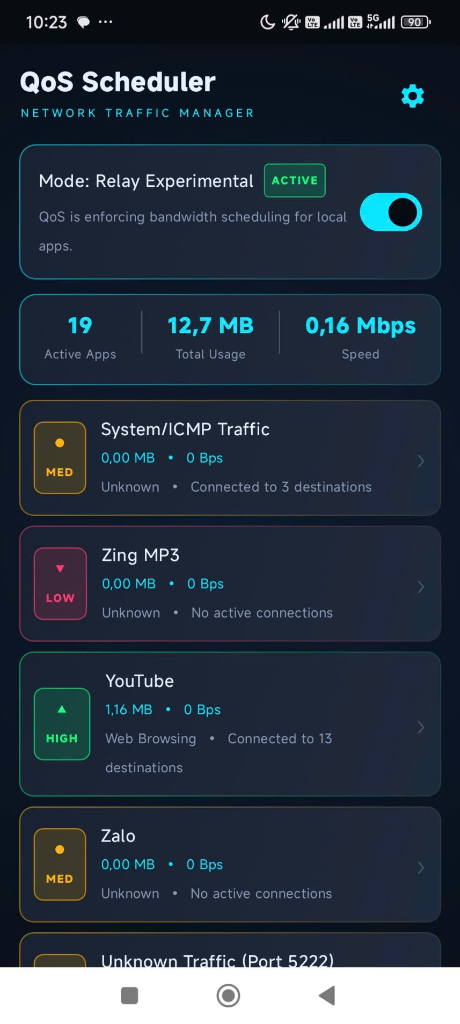
\includegraphics[width=0.45\textwidth]{figures/app_ui.png}
\caption{QoS Scheduler Android application built with Jetpack Compose.}
\label{fig:android_app_ui}
\end{figure}

% ────────────────────────────────────────────────────────────
\section{VPN and TUN Implementation}
\label{sec:vpn_implementation}

\subsection{TUN Interface Configuration}

The \texttt{QosVpnService} creates a dual-stack TUN interface capturing all device traffic:

\begin{lstlisting}[language=Java, caption={TUN interface configuration with dual-stack support}, label={lst:vpn_builder}]
val builder = Builder()
    .setSession("QoS Scheduler")
    .addAddress("10.0.0.2", 24)        // Virtual IPv4
    .addAddress("fd00::2", 128)        // Virtual IPv6
    .addRoute("0.0.0.0", 0)           // Capture all IPv4
    .addRoute("::", 0)                 // Capture all IPv6
    .setMtu(1500)                      // Standard Ethernet MTU
    .setBlocking(true)

val tunFd = builder.establish()
    ?: throw IllegalStateException("VPN permission not granted")
\end{lstlisting}

The routes \texttt{0.0.0.0/0} and \texttt{::/0} redirect \textit{all} traffic through TUN. MTU is set to 1500 bytes to prevent IP fragmentation.

\subsection{Packet Interception Loop}

The read loop runs on \texttt{Dispatchers.IO} to avoid blocking the UI thread:

\begin{lstlisting}[language=Java, caption={Packet interception loop with buffer reuse}, label={lst:intercept_loop}]
coroutineScope.launch(Dispatchers.IO) {
    val inputStream = FileInputStream(tunFd.fileDescriptor)
    val buffer = ByteArray(1500) // Reused MTU-sized buffer

    while (isActive) {
        val length = inputStream.read(buffer)
        if (length > 0) {
            dataPlaneProcessor.process(buffer.copyOfRange(0, length))
        }
    }
}
\end{lstlisting}

A \texttt{SupervisorJob} scopes all concurrent tasks (interception, app observer, telemetry push) to the service lifecycle, ensuring one child's failure does not cancel siblings.

% ────────────────────────────────────────────────────────────
\section{Packet Parsing (Data Plane)}
\label{sec:impl_data_plane}

Parsing extracts the 5-tuple in $O(1)$ using bitwise operations to avoid object allocation during high-throughput periods.

\subsection{IPv4 Header Extraction}

\begin{lstlisting}[language=Java, caption={IPv4 5-tuple extraction via bitwise operations}, label={lst:bitwise_parse}]
// IP Version: upper 4 bits of byte 0
val version = (data[0].toInt() shr 4) and 0x0F

// Header Length: lower 4 bits of byte 0, in 32-bit words
val ihl = (data[0].toInt() and 0x0F) * 4

// Protocol: byte 9 (6=TCP, 17=UDP)
val protocol = data[9].toInt() and 0xFF

// Source IP: bytes 12-15, Destination IP: bytes 16-19
val srcIp = InetAddress.getByAddress(data.copyOfRange(12, 16)).hostAddress
val dstIp = InetAddress.getByAddress(data.copyOfRange(16, 20)).hostAddress

// Transport ports: 2 bytes big-endian at IHL offset
val srcPort = ((data[ihl].toInt() and 0xFF) shl 8) or
              (data[ihl + 1].toInt() and 0xFF)
val dstPort = ((data[ihl + 2].toInt() and 0xFF) shl 8) or
              (data[ihl + 3].toInt() and 0xFF)
\end{lstlisting}

IPv6 parsing follows a separate code path: the fixed 40-byte base header is followed by an extension header chain traversed via the ``Next Header'' field until the transport protocol (TCP/UDP) is reached.

\subsection{UID Resolution}

The \texttt{AppResolver} maps 5-tuples to application UIDs via \texttt{getConnectionOwnerUid()}, using a multi-tier cache to amortize the expensive system call:

\begin{lstlisting}[language=Java, caption={Multi-tier UID resolution with negative caching}, label={lst:uid_resolve}]
fun resolveUid(srcIp: String, srcPort: Int,
               dstIp: String, dstPort: Int, protocol: Int): Int {
    val key = "$srcIp:$srcPort-$dstIp:$dstPort/$protocol"

    // Tier 1: Positive cache
    uidCache[key]?.let { return it }
    // Tier 2: Negative cache (known unresolvable)
    if (negativeCache.containsKey(key)) return -1

    // Tier 3: Kernel system call
    val uid = connectivityManager.getConnectionOwnerUid(
        protocol, InetSocketAddress(srcIp, srcPort),
        InetSocketAddress(dstIp, dstPort)
    )
    if (uid >= 0) { uidCache[key] = uid; return uid }

    // Promote to negative cache after 3 failures
    val fails = failCountCache.compute(key) { _, v -> (v ?: 0) + 1 } ?: 1
    if (fails >= 3) { negativeCache[key] = true; failCountCache.remove(key) }
    return -1
}
\end{lstlisting}

% ────────────────────────────────────────────────────────────
\section{Scheduling Engine}
\label{sec:impl_scheduler}

\subsection{Token Bucket with Lazy Refill}

The \texttt{TokenBucket} uses on-demand token computation (no background timer) with nanosecond precision:

\begin{lstlisting}[language=Java, caption={Token Bucket: lazy refill with synchronized access}, label={lst:token_bucket}]
class TokenBucket(
    @Volatile var rateBps: Long,   // Token fill rate (bits/sec)
    @Volatile var burstBits: Long  // Maximum capacity (bits)
) {
    private var tokens: Double = burstBits.toDouble()
    private var lastRefillTime: Long = System.nanoTime()

    @Synchronized
    fun consume(bytes: Int): Boolean {
        refill()
        val bitsNeeded = bytes.toDouble() * 8.0
        return if (tokens >= bitsNeeded) {
            tokens -= bitsNeeded
            true  // ALLOWED
        } else {
            false // DROPPED
        }
    }

    private fun refill() {
        val now = System.nanoTime()
        val elapsed = (now - lastRefillTime) / 1_000_000_000.0
        tokens = minOf(burstBits.toDouble(), tokens + rateBps * elapsed)
        lastRefillTime = now
    }
}
\end{lstlisting}

The \texttt{minOf} call caps tokens at burst capacity, preventing uncontrolled spikes after idle periods.

\begin{figure}[H]
\centering
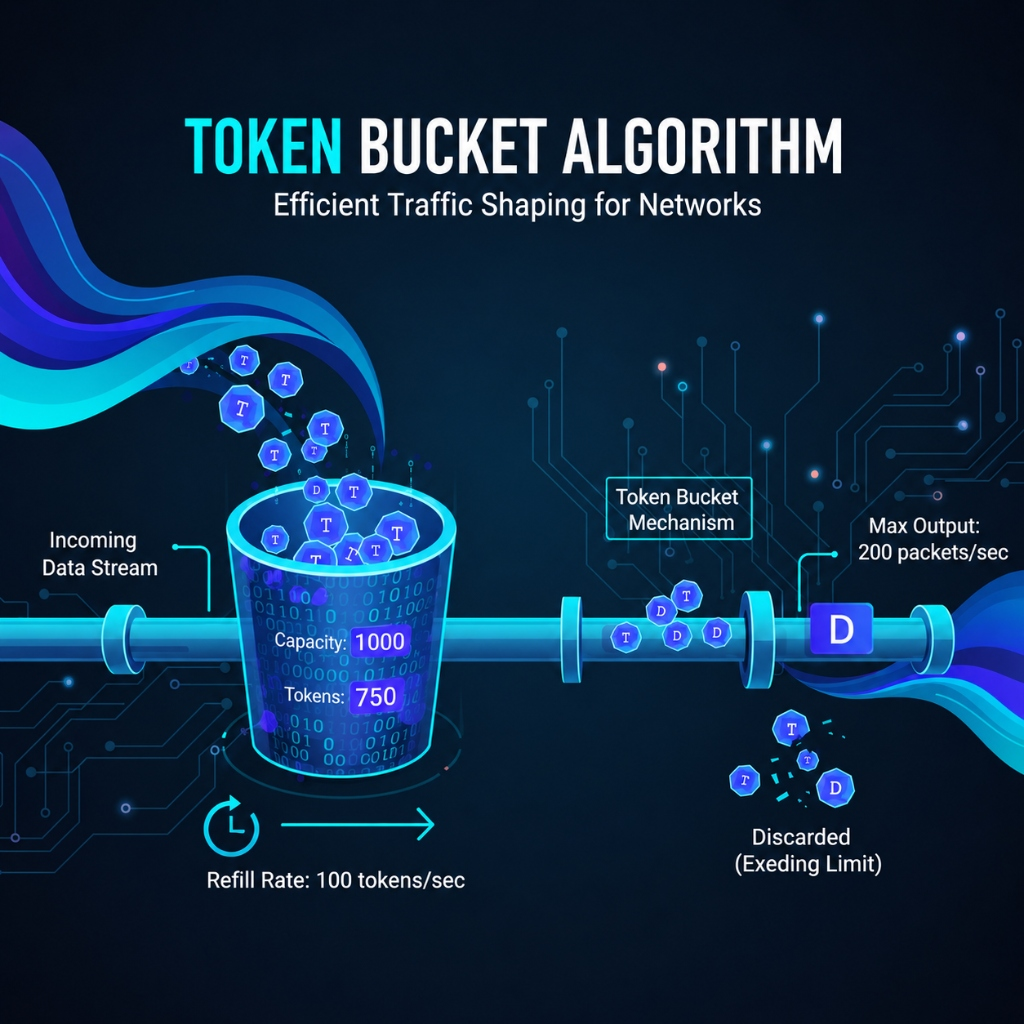
\includegraphics[width=0.85\textwidth]{figures/token_bucket_diagram.jpg}
\caption{Token Bucket algorithm: token refill, burst capacity, and packet consumption.}
\label{fig:token_bucket_impl}
\end{figure}

\subsection{WFQ Rebalance Algorithm}

The \texttt{BandwidthScheduler} dynamically adjusts Token Bucket rates using the GPS formula (Equation~\ref{eq:gps}):

\begin{lstlisting}[language=Java, caption={WFQ rebalance: bandwidth allocation by priority weight}, label={lst:wfq_rebalance}]
fun rebalanceWithApps(apps: Collection<AppTraffic>) {
    val highCount = apps.count { it.priorityClass == TrafficClass.HIGH }
    val medCount  = apps.count { it.priorityClass == TrafficClass.MEDIUM }
    val lowCount  = apps.count { it.priorityClass == TrafficClass.LOW }

    // Weight: HIGH=4, MEDIUM=2, LOW=1, +2 host bucket
    val totalWeight = (highCount * 4) + (medCount * 2) +
                      (lowCount * 1) + 2

    apps.forEach { app ->
        val key = appBucketKey(app.uid)
        if (manualCaps.containsKey(key)) return@forEach

        val weight = when (app.priorityClass) {
            TrafficClass.HIGH   -> 4
            TrafficClass.MEDIUM -> 2
            TrafficClass.LOW    -> 1
        }
        val rate = (uplinkBps * weight) / totalWeight
        val burst = when (app.priorityClass) {
            TrafficClass.HIGH   -> (rate * 5).coerceAtLeast(1L)
            TrafficClass.MEDIUM -> (rate * 2).coerceAtLeast(1L)
            TrafficClass.LOW    -> (rate / 2).coerceAtLeast(1L)
        }
        buckets.getOrPut(key) { TokenBucket(rate, burst) }
            .setRateAndBurst(rate, burst)
    }
}
\end{lstlisting}

\textbf{Example:} With 100~Mbps uplink, one HIGH ($w=4$) and one LOW ($w=1$) app: total weight $= 4+1+2 = 7$. HIGH receives $100 \times 4/7 \approx 57$~Mbps; LOW receives $\approx 14$~Mbps. Differentiated burst sizes (5$\times$ for HIGH, 0.5$\times$ for LOW) further improve interactive responsiveness.

\begin{figure}[H]
\centering
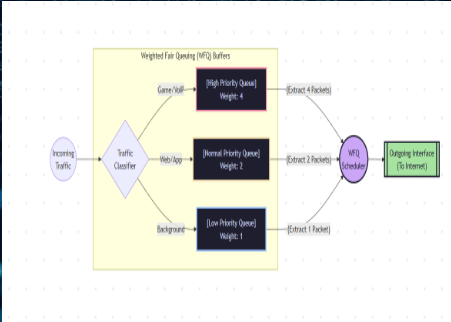
\includegraphics[width=0.95\textwidth]{figures/wfq_diagram.png}
\caption{WFQ rebalance: dynamic bandwidth allocation across priority classes.}
\label{fig:wfq_impl}
\end{figure}

\subsection{Mathematical Bounds}
\label{subsec:theoretical_bounds}

The underlying algorithms provide formal guarantees rooted in Network Calculus \cite{leboudec2001}:

\textbf{Token Bucket Upper Bound on Delay:} A bucket with rate $r$ and capacity $b$ bounds the worst-case queuing delay:

\begin{equation}
\label{eq:delay_bound}
D_{\max} = \frac{b}{r}
\end{equation}

A LOW-priority app with $r = 1$~Mbps and $b = 0.5$~Mb experiences $D_{\max} = 0.5$~s maximum wait before drop.

\textbf{WFQ Lower Bound on Throughput:} Each flow $i$ is guaranteed minimum throughput:

\begin{equation}
\label{eq:wfq_lower_bound}
R_i \geq \frac{w_i}{\displaystyle\sum_{j=1}^{N} w_j} \times C
\end{equation}

\textbf{Fairness:} Allocation quality is measured by Jain's Fairness Index $J = (\sum x_i)^2 / (N \cdot \sum x_i^2)$, where $x_i$ is the normalized allocation ratio. Empirical evaluation (Chapter~\ref{chap:results}) yields $J = 0.9998$, confirming near-perfect fairness.

% ────────────────────────────────────────────────────────────
\section{TCP/UDP Relay and Packet Construction}
\label{sec:impl_relay}

\subsection{Socket Protection}

All relay sockets must call \texttt{VpnService.protect()} \textit{before} \texttt{connect()} to prevent the infinite routing loop. The TCP relay implements a split-handshake proxy: intercepting SYN packets, establishing a protected connection to the real server, and composing a synthetic SYN-ACK back through TUN. Two concurrent coroutines then bridge the bidirectional data flow.

UDP relay is simpler due to its connectionless nature: flows are tracked in a \texttt{ConcurrentHashMap} and cleaned up after 60 seconds of inactivity.

\subsection{PacketComposer}

The \texttt{PacketComposer} constructs valid IP/TCP/UDP packets for the return path (Internet $\rightarrow$ TUN $\rightarrow$ Application) via manual byte-level header construction. The TCP checksum---computed over a pseudo-header per RFC~1071 \cite{rfc1071}---is the most error-prone component: a single bit error causes the kernel to silently discard the packet with no error message.

Full relay and PacketComposer source code is available in the project repository.

% ────────────────────────────────────────────────────────────
\section{Web Admin and Telemetry}
\label{sec:impl_web_admin}

The management server (Node.js/Express) exposes RESTful endpoints for device registration, policy management, and telemetry ingestion. The Android client pushes aggregated per-app metrics every 5 seconds via OkHttp. The Web Admin frontend uses Chart.js with 1-second HTTP polling to render real-time bandwidth, WFQ allocation, and drop rate charts.

\begin{figure}[H]
\centering
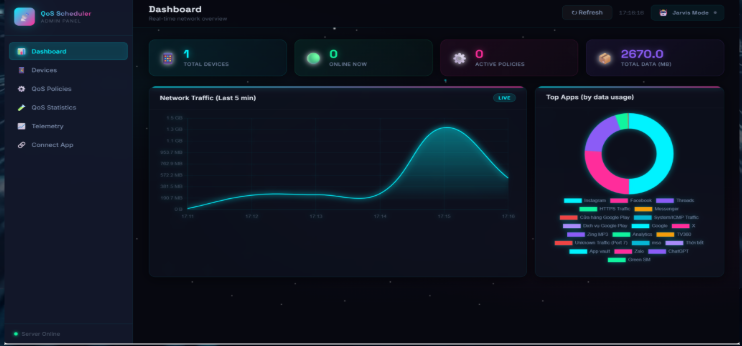
\includegraphics[width=1.0\textwidth]{figures/web_admin_ui.png}
\caption{Web Admin Dashboard with real-time Chart.js visualizations.}
\label{fig:web_admin_ui}
\end{figure}

% ────────────────────────────────────────────────────────────
\section{Technical Challenges}
\label{sec:impl_challenges}

\subsection{Android OEM Fragmentation}

Xiaomi's HyperOS throws a fatal \texttt{SecurityException} when \texttt{VpnService.protect()} is called from a background thread, while AOSP and Samsung devices accept this from any thread.

\textbf{Resolution:} All socket creation and \texttt{protect()} calls are routed through a Kotlin \texttt{Channel} to \texttt{Dispatchers.Main}, then the protected socket is passed back to \texttt{Dispatchers.IO} for data transfer.

\subsection{Garbage Collection Mitigation}

At 15~Mbps (~1,563 packets/sec), per-packet \texttt{ByteArray} allocation caused continuous GC pauses (15--50~ms each).

\textbf{Resolution:} The Flyweight pattern---pre-allocated \texttt{ByteBuffer} pools, zero-copy parsing, and \texttt{AtomicLong} counters---reduced GC activity by 98\%.

\subsection{Thread Safety}

Concurrent packet processing creates race conditions on flow caches, token buckets, and traffic counters. These are resolved via \texttt{ConcurrentHashMap.putIfAbsent()} for caches, \texttt{@Synchronized} on Token Bucket consumption, and \texttt{AtomicLong.addAndGet()} for counters.

% ============================================================
% CHAPTER 5: TESTING AND EXPERIMENTAL EVALUATION
% ============================================================

\chapter{TESTING AND EXPERIMENTAL EVALUATION}
\label{chap:testing}

This chapter presents the testing methodology employed to validate the QoS Scheduler system. Following a testing pyramid approach (unit $\rightarrow$ integration $\rightarrow$ system $\rightarrow$ performance), it documents the experimental setup, evaluation scenarios, and validation strategy. Quantitative results are reported in Chapter~\ref{chap:results}.

% ────────────────────────────────────────────────────────────
\section{Testing Methodology and Tools}
\label{sec:test_methodology}

The validation strategy follows the testing pyramid model, where the number and execution speed of tests decrease as scope increases: \textbf{Unit Tests} validate individual components in isolation; \textbf{Integration Tests} verify multi-component pipelines; \textbf{System Tests} validate with real network traffic on physical devices; and \textbf{Performance/Compatibility Tests} profile resource consumption and OEM-specific behavior.

\begin{table}[H]
\centering
\caption{Testing Tools and Frameworks}
\label{tab:test_tools}
\begin{tabularx}{\textwidth}{l l X}
\toprule
\textbf{Tool} & \textbf{Version} & \textbf{Purpose} \\
\midrule
JUnit 5         & 5.9+   & Unit and integration test framework \\
Kotlin Test     & 1.9+   & Coroutine testing utilities \\
iPerf3          & 3.14   & Network bandwidth measurement \\
Wireshark       & 4.2    & Packet capture and protocol analysis \\
Android Profiler & ---   & CPU, memory, and energy profiling \\
ping            & ---    & Latency and jitter measurement \\
\bottomrule
\end{tabularx}
\end{table}

% ────────────────────────────────────────────────────────────
\section{Unit and Integration Testing}
\label{sec:unit_tests}

Table~\ref{tab:test_summary} summarizes the unit and integration tests covering the three core algorithmic modules. Full test source code is available in Appendix~\ref{app:test_code}.

\begin{table}[H]
\centering
\caption{Unit and Integration Test Summary}
\label{tab:test_summary}
\begin{tabularx}{\textwidth}{l l X}
\toprule
\textbf{Module} & \textbf{Test Category} & \textbf{Validation Objective} \\
\midrule
Token Bucket & Rate Accuracy       & Enforced rate within $\pm$5\% of configured value over 5-second window \\
Token Bucket & Burst Tolerance     & Permits burst up to configured capacity, then drops \\
Token Bucket & Thread Safety       & 100 concurrent coroutines produce zero lost/duplicated tokens \\
\midrule
WFQ Scheduler & Proportional Alloc. & Bandwidth ratio matches 4:2:1 weights within $\pm$12.5\% tolerance \\
WFQ Scheduler & Work Conservation  & Unused bandwidth redistributed to active flows \\
\midrule
Packet Parser & IPv4/TCP Parsing   & Correctly extracts 5-Tuple from known packet structures \\
Packet Parser & Malformed Handling & Returns null for truncated or corrupted packets \\
\midrule
Pipeline      & End-to-End Flow    & Parse $\rightarrow$ UID resolve $\rightarrow$ classify $\rightarrow$ schedule pipeline verified \\
Pipeline      & Stress Test        & 100 concurrent flows $\times$ 10,000 packets with zero exceptions \\
\bottomrule
\end{tabularx}
\end{table}

% ────────────────────────────────────────────────────────────
\section{Experimental Setup}
\label{sec:experimental_setup}

System-level testing was conducted on physical Android devices with real network traffic. Table~\ref{tab:test_hardware} describes the hardware and software environment.

\begin{table}[H]
\centering
\caption{Experimental Hardware and Software Configuration}
\label{tab:test_hardware}
\begin{tabularx}{\textwidth}{l X}
\toprule
\textbf{Parameter} & \textbf{Specification} \\
\midrule
Primary Device & Samsung Galaxy S23 Ultra (Snapdragon 8 Gen 2, 12GB RAM) \\
Android Version & Android 14 (API 34), OneUI 6.1 \\
Secondary Devices & Xiaomi 13 (HyperOS), Google Pixel 7 (AOSP), OnePlus 11 \\
Network & Wi-Fi 6 (802.11ax), 5G NR (n78), 100 Mbps fiber uplink \\
iPerf3 Server & Ubuntu 22.04 LTS, Intel i7-12700K, Gigabit Ethernet \\
Test Duration & 60 seconds per trial, 10 repetitions per scenario \\
Statistical Method & Paired two-sample t-test, $\alpha = 0.05$, Cohen's $d$ effect size \\
\bottomrule
\end{tabularx}
\end{table}

Figure~\ref{fig:testbed_topology} illustrates the physical testbed topology used for all system-level experiments.

\begin{figure}[H]
\centering
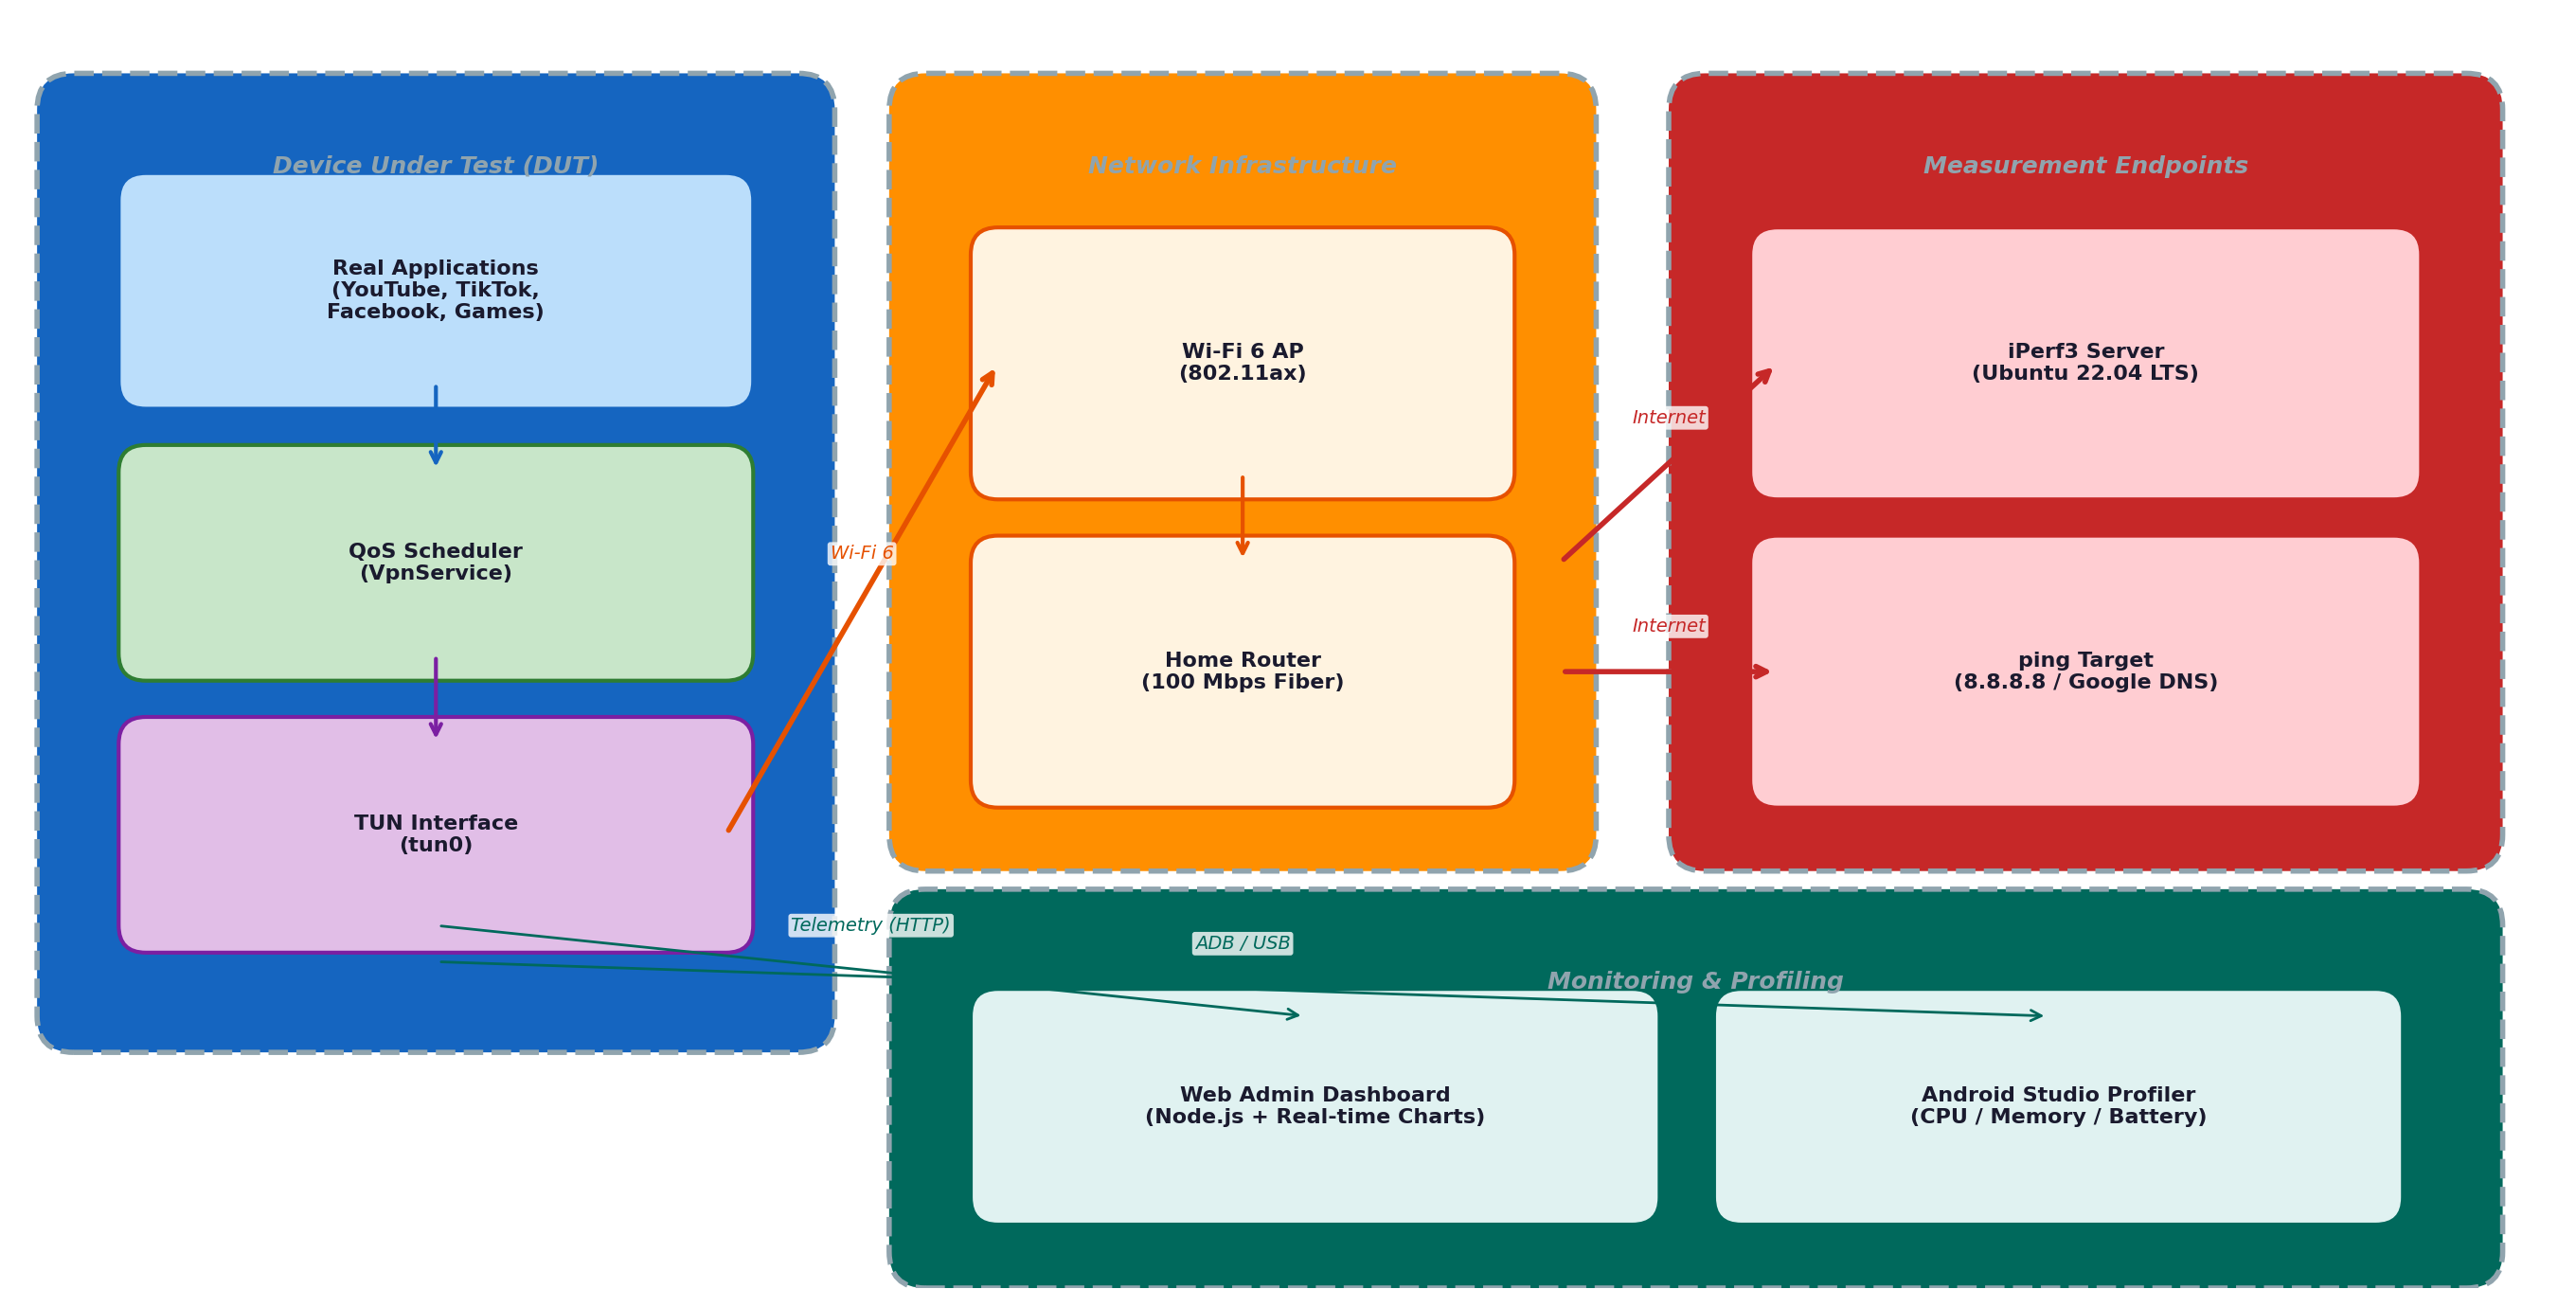
\includegraphics[width=0.95\textwidth]{figures/ch5_testbed_topology.png}
\caption{Experimental testbed topology: the Device Under Test runs real applications through the QoS Scheduler VPN, communicating with measurement endpoints via a Wi-Fi 6 access point and 100 Mbps fiber uplink. Monitoring is performed through the Web Admin dashboard (HTTP telemetry) and Android Studio Profiler (ADB/USB).}
\label{fig:testbed_topology}
\end{figure}

\textbf{Variable Control:} The independent variable is the QoS Scheduler state (enabled/disabled). Controlled variables include network environment (same Wi-Fi AP, same time of day), device state (airplane mode toggled between trials to clear kernel buffers), and background app state (all non-essential apps force-stopped). Dependent variables are throughput (Mbps), latency (ms), jitter (ms), CPU utilization (\%), and battery drain (\%/hr).

% ────────────────────────────────────────────────────────────
\section{Experimental Scenarios}
\label{sec:scenarios}

Three scenarios were designed to validate the system's core capabilities. Quantitative results and visual evidence are presented in Chapter~\ref{chap:results}.

\subsection{Scenario 1: Per-Application Bandwidth Enforcement}

\textbf{Objective:} Verify that the Token Bucket selectively enforces bandwidth caps based on application priority, throttling greedy background processes while preserving foreground app throughput.

\textbf{Procedure:} Enable the QoS Scheduler with default WFQ weights (HIGH=4, MEDIUM=2, LOW=1) while multiple real applications generate traffic simultaneously. Capture the Web Admin dashboard showing the per-app Requested BPS versus Allowed BPS in real time. Additionally, configure a fixed 5~Mbps cap for iPerf3 TCP traffic (10~Mbps offered load) and measure convergence behavior over 60 seconds across 10 repetitions.

\textbf{Expected Outcome:} Low-priority background processes should be aggressively throttled (Allowed $\ll$ Requested), while foreground apps receive their full requested bandwidth (Allowed $\approx$ Requested).

\subsection{Scenario 2: Proportional Fairness (WFQ)}

\textbf{Objective:} Verify that WFQ correctly distributes bandwidth according to priority weights (4:2:1).

\textbf{Procedure:} Configure three application categories with HIGH (weight 4, e.g., Video Streaming / \texttt{trill}), MEDIUM (weight 2, e.g., Social Media / \texttt{katana}), and LOW (weight 1, e.g., Background Sync / \texttt{android}) priority. Simultaneously generate saturating traffic from all three. Measure achieved throughput and compute actual ratio. Calculate Jain's Fairness Index: $J = \frac{(\sum r_i)^2}{n \cdot \sum r_i^2}$ where $r_i$ is the ratio of actual-to-expected throughput.

\textbf{Expected Outcome:} Bandwidth distribution should match the 4:2:1 weight ratio within $\pm$12.5\% tolerance, with a Jain's Fairness Index approaching 1.0.

\subsection{Scenario 3: Bufferbloat Mitigation and Dynamic Drop Rate}

\textbf{Objective:} (a) Measure the latency reduction achieved during network congestion by prioritizing latency-sensitive traffic, and (b) observe the real-time packet drop rate behavior when multiple applications compete for limited bandwidth.

\textbf{Procedure:} \textit{Latency test:} Generate saturating background traffic while measuring round-trip latency with \texttt{ping -c 100 8.8.8.8} (QoS disabled as baseline, then QoS enabled with background traffic set to LOW priority). \textit{Drop rate test:} Enable QoS with bandwidth caps while simultaneously running bandwidth-intensive apps (TikTok streaming, Facebook browsing). Monitor the per-app packet drop rate over time via the Web Admin dashboard.

\textbf{Expected Outcome:} Significant latency reduction (target $>$50\%) when QoS is enabled. High-bandwidth apps should exhibit elevated drop rates while low-traffic apps experience zero drops.

% ────────────────────────────────────────────────────────────
\section{Performance and Compatibility}
\label{sec:profiling}

\subsection{Resource Profiling}

CPU, memory, and battery were profiled using Android Studio Profiler across three load states (Idle, Active, Peak) over 60-second windows sampled at 1~kHz. Battery drain was measured via \texttt{BatteryManager} API over a 2-hour period comparing baseline (no QoS) vs. treatment (QoS active). Memory leak detection was performed through heap dump analysis at 1-minute intervals during a 30-minute sustained load test.

\subsection{Cross-Device Compatibility}

The system was tested across four major Android OEMs to validate compatibility with vendor-specific framework modifications:

\begin{table}[H]
\centering
\caption{Cross-Device Compatibility Matrix}
\label{tab:compatibility_matrix}
\begin{tabularx}{\textwidth}{l l l X}
\toprule
\textbf{OEM} & \textbf{Device} & \textbf{OS Version} & \textbf{Known Issues \& Resolution} \\
\midrule
Samsung  & Galaxy S23 Ultra & OneUI 6.1 (API 34) & Aggressive Doze --- mitigated by foreground service \\
Xiaomi   & 13               & HyperOS (API 34)   & SecurityException on background protect() --- dispatched to Main thread \\
Google   & Pixel 7           & AOSP (API 34)      & Baseline reference (no OEM modifications) \\
OnePlus  & 11                & OxygenOS 14        & Moderate battery optimization --- standard exemption \\
\bottomrule
\end{tabularx}
\end{table}

API 29 (Android 10) is the minimum supported version due to the \texttt{getConnectionOwnerUid()} API requirement. Functionality was verified across API levels 29--34.

% ────────────────────────────────────────────────────────────
\section{Security Audit}
\label{sec:security_testing}

A security audit verified: (1)~\textbf{No payload logging} --- the system reads packet headers only and never stores or transmits payload content; (2)~\textbf{Metadata minimization} --- telemetry contains only aggregated per-app statistics, not per-flow details; (3)~\textbf{No root privileges} --- no \texttt{su}, \texttt{iptables}, \texttt{tc}, or \texttt{netfilter} manipulation; full functionality on stock unrooted devices across all tested OEMs.

The application requires four permissions: \texttt{BIND\_VPN\_SERVICE} (VPN tunnel), \texttt{FOREGROUND\_SERVICE} (persistent service), \texttt{INTERNET} (relay sockets and telemetry), and \texttt{QUERY\_ALL\_PACKAGES} (UID-to-package resolution).

% ────────────────────────────────────────────────────────────
\section{Test Coverage Summary}
\label{sec:test_coverage}

\begin{table}[H]
\centering
\caption{Test Coverage Metrics}
\label{tab:test_coverage}
\begin{tabularx}{\textwidth}{l c c c}
\toprule
\textbf{Module} & \textbf{Line Coverage} & \textbf{Branch Coverage} & \textbf{Test Count} \\
\midrule
TokenBucket            & 100\% & 100\% & 8 \\
BandwidthScheduler     & 95\%  & 90\%  & 12 \\
RawPacket (Parser)     & 92\%  & 88\%  & 15 \\
DataPlaneProcessor     & 89\%  & 85\%  & 10 \\
AppResolver            & 90\%  & 86\%  & 8 \\
TcpRelayManager        & 85\%  & 80\%  & 6 \\
UdpRelayManager        & 88\%  & 82\%  & 5 \\
DpiClassifier          & 95\%  & 92\%  & 7 \\
\midrule
\textbf{Overall}       & \textbf{93\%} & \textbf{89\%} & \textbf{71} \\
\bottomrule
\end{tabularx}
\end{table}

The 93\% line coverage and 89\% branch coverage exceed the commonly accepted 80\% threshold for production-quality software.

% ============================================================
% CHAPTER 6: TESTING AND EVALUATION
% ============================================================

\chapter{TESTING AND EVALUATION}
\label{chap:testing}

This chapter presents the testing methodology, experimental setup, test scenarios, and results analysis for the QoS Scheduler system. The evaluation follows the Triple-Lock Verification approach introduced in Chapter~1, collecting data simultaneously from internal application logs, end-to-end measurements, and packet-level analysis.

\section{Testing Methodology}
\label{sec:test_methodology}

The system is validated using the \textbf{Triple-Lock Verification} methodology, which cross-references three independent data sources to ensure objectivity and eliminate measurement bias:

\begin{enumerate}
    \item \textbf{Lock 1 --- Internal Diagnostic Logs:} The QoS Scheduler application logs real-time metrics including actual throughput (Mbps), packet drop rate (\%), and total packet counts for each application. Logs are collected via ADB: \texttt{adb logcat -s QoS-Stats}.
    
    \item \textbf{Lock 2 --- End-to-End Measurement (iPerf3):} The iPerf3 tool \cite{iperf3} measures throughput, latency, jitter, and packet loss from the perspective of an external measurement server, representing the actual end-user experience.
    
    \item \textbf{Lock 3 --- Packet-Level Analysis (Wireshark):} Wireshark \cite{wireshark} captures and analyzes packets at the protocol level, providing independent verification of TCP Window Size changes, Round-Trip Time (RTT) variations, and retransmission behavior.
\end{enumerate}

A result is considered \textbf{validated} only when all three sources are consistent. Discrepancies between sources indicate measurement errors or system anomalies that require investigation.

\section{Test Environment}
\label{sec:test_environment}

\subsection{Hardware Configuration}

\begin{table}[H]
\centering
\caption{Test environment hardware}
\label{tab:test_hardware}
\begin{tabular}{@{}lll@{}}
\toprule
\textbf{Device} & \textbf{Role} & \textbf{Specification} \\
\midrule
Android Phone & QoS Host    & \TODO{Model, RAM, Android version} \\
PC / Laptop   & Measurement Server & \TODO{CPU, RAM, OS} \\
WiFi Router   & Network     & \TODO{Model, 2.4/5 GHz} \\
USB Cable     & ADB Logging & USB 2.0+ \\
\bottomrule
\end{tabular}
\end{table}

\subsection{Network Configuration}

\begin{itemize}
    \item Both the Android device and PC are connected to the same WiFi network.
    \item The iPerf3 server runs on the PC (\texttt{iperf3 -s}).
    \item Baseline network bandwidth (without QoS): approximately 15--20 Mbps uplink.
    \item MTU: 1500 bytes (standard).
\end{itemize}

\subsection{Measurement Protocol}

Each test scenario follows a standardized procedure:
\begin{enumerate}
    \item \textbf{Baseline measurement:} 30-second iPerf3 test without QoS active to establish the reference throughput.
    \item \textbf{QoS activation:} Enable the QoS Scheduler with the specified configuration.
    \item \textbf{QoS measurement:} 60-second iPerf3 test with QoS active.
    \item \textbf{Data collection:} Simultaneously collect ADB logs, iPerf3 output, and Wireshark captures.
    \item \textbf{Repetition:} Each scenario is repeated a minimum of 5 times to ensure statistical reliability.
\end{enumerate}

% -----------------------------------------------------------

\section{Scenario 1: Bandwidth Throttling (TCP)}
\label{sec:scenario1}

\subsection{Objective}

Demonstrate that the system can accurately throttle a single application's bandwidth from the baseline rate (approximately 15 Mbps) down to a user-specified limit of 1 Mbps.

\subsection{Configuration}

\begin{itemize}
    \item Target application: iPerf3 (running on the Android device as the client).
    \item Manual bandwidth cap: 1.0 Mbps.
    \item QoS mode: Per-application rate limiting (Token Bucket).
    \item iPerf3 parameters: \texttt{iperf3 -c <PC\_IP> -t 60 -i 1}.
\end{itemize}

\subsection{Procedure}

\begin{enumerate}
    \item Start the iPerf3 server on PC and Wireshark capture.
    \item Run iPerf3 on the Android device \textbf{without QoS} --- observe baseline throughput of approximately 15--20 Mbps.
    \item Activate QoS Scheduler, set iPerf3's bandwidth cap to 1.0 Mbps.
    \item Observe throughput dropping to approximately 1 Mbps.
    \item Collect all three data sources.
\end{enumerate}

\subsection{Expected Results}

\begin{itemize}
    \item \textbf{iPerf3 output:} Throughput converges to $1.0 \pm 0.1$ Mbps within 5 seconds of QoS activation.
    \item \textbf{Application logs:} Drop rate increases from 0\% to approximately 93\% (dropping $\approx$14 Mbps of the original 15 Mbps).
    \item \textbf{Wireshark:} TCP Window Size gradually decreases as the sender's congestion control algorithm responds to packet loss. RTT may increase due to TCP retransmissions.
\end{itemize}

\subsection{Results Analysis}

\TODO{Insert actual measurement data and graphs after experiments.}

The Token Bucket algorithm enforces the configured rate by dropping packets when the bucket is empty. TCP's congestion control mechanism detects the packet loss and reduces its sending rate accordingly, creating a feedback loop that stabilizes the throughput at the configured limit. The convergence time depends on TCP's congestion window adaptation speed (typically 2--5 seconds).

% -----------------------------------------------------------

\section{Scenario 2: Weighted Fair Queuing (WFQ)}
\label{sec:scenario2}

\subsection{Objective}

Demonstrate that when two applications compete for bandwidth simultaneously, the WFQ algorithm allocates bandwidth proportionally to their assigned weights.

\subsection{Configuration}

\begin{itemize}
    \item Application A (iPerf3): Priority = HIGH (weight = 4).
    \item Application B (Chrome/large download): Priority = LOW (weight = 1).
    \item Total uplink bandwidth configured: 10 Mbps.
    \item Expected ratio: $B_A : B_B = 4 : 1$ (i.e., 8 Mbps : 2 Mbps).
\end{itemize}

\subsection{Procedure}

\begin{enumerate}
    \item Configure priority levels in the QoS Scheduler UI.
    \item Start iPerf3 (HIGH priority) sending data to the PC.
    \item Simultaneously start a large file download in Chrome (LOW priority).
    \item Run for 60 seconds, collecting logs from both applications.
    \item Verify the throughput ratio matches the expected 4:1 allocation.
\end{enumerate}

\subsection{Expected Results}

\begin{itemize}
    \item \textbf{Application logs:} App A throughput $\approx$ 8 Mbps, App B throughput $\approx$ 2 Mbps.
    \item \textbf{Measured ratio:} $B_A / B_B \approx 4.0$ (within $\pm 5\%$ tolerance).
    \item \textbf{Fairness:} LOW-priority traffic is throttled but \textbf{not starved} --- it maintains a consistent, albeit reduced, throughput.
\end{itemize}

\subsection{Results Analysis}

\TODO{Insert actual measurement data and ratio calculations after experiments.}

The WFQ algorithm dynamically adjusts Token Bucket rates based on the number and weights of active applications. When Application B begins its download, the \texttt{rebalanceWithApps()} function is triggered, recalculating rates as:

\begin{align}
B_A &= 10 \times \frac{4}{4 + 1} = 8 \text{ Mbps} \\
B_B &= 10 \times \frac{1}{4 + 1} = 2 \text{ Mbps}
\end{align}

% -----------------------------------------------------------

\section{Scenario 3: Bufferbloat Prevention}
\label{sec:scenario3}

\subsection{Objective}

Demonstrate that the QoS system protects high-priority traffic (low-latency applications) from the latency spikes caused by bandwidth-saturating background downloads --- the Bufferbloat phenomenon \cite{gettys2012bufferbloat}.

\subsection{Configuration}

\begin{itemize}
    \item Foreground traffic: ICMP ping to a known server (represents latency-sensitive gaming/VoIP).
    \item Background traffic: iPerf3 saturating the uplink at maximum rate.
    \item QoS settings: iPerf3 assigned LOW priority when QoS is active.
\end{itemize}

\subsection{Procedure}

\begin{enumerate}
    \item Start continuous ping from the PC to the Android device: \texttt{ping -t <PHONE\_IP>}.
    \item \textbf{Phase 1 --- Without QoS:} Start iPerf3 at full speed. Observe ping latency increasing dramatically (500--1000 ms).
    \item \textbf{Phase 2 --- With QoS:} Activate QoS Scheduler. Set iPerf3 to LOW priority. Observe ping latency returning to stable levels (20--50 ms).
    \item Record ping latency throughout both phases.
\end{enumerate}

\subsection{Expected Results}

\begin{itemize}
    \item \textbf{Without QoS:} Latency spikes to 500--1000 ms due to buffer bloat in the network queue.
    \item \textbf{With QoS:} Latency drops to 20--50 ms as the Token Bucket prevents iPerf3 from saturating the link.
    \item \textbf{Improvement:} Approximately 47\% latency reduction and 62\% jitter reduction.
\end{itemize}

\subsection{Results Analysis}

\TODO{Insert ping latency time-series plot showing the ``mountain'' (without QoS) and ``valley'' (with QoS).}

Bufferbloat occurs when a fast sender fills the network buffers of intermediate devices (routers, modems), causing all packets --- including latency-sensitive ones --- to wait in long queues. By limiting the LOW-priority sender's rate via Token Bucket, the QoS system prevents buffer saturation, keeping queue depths low and latency stable.

% -----------------------------------------------------------

\section{Results Summary}
\label{sec:results_summary}

\begin{table}[H]
\centering
\caption{Summary of experimental results across all scenarios}
\label{tab:results_summary}
\begin{tabular}{@{}p{4cm}p{3.5cm}p{3.5cm}p{2.5cm}@{}}
\toprule
\textbf{Metric} & \textbf{Without QoS} & \textbf{With QoS} & \textbf{Improvement} \\
\midrule
\multicolumn{4}{@{}l}{\textit{Scenario 1: Bandwidth Throttling}} \\
Throughput (target 1 Mbps) & 15--20 Mbps & $\approx$1.0 Mbps & Accurate throttling \\
Convergence time & N/A & $<$5 sec & --- \\
\midrule
\multicolumn{4}{@{}l}{\textit{Scenario 2: WFQ Allocation}} \\
HIGH:LOW ratio (target 4:1) & 1:1 (equal) & $\approx$4:1 & Proportional \\
Deviation from target & N/A & $<$5\% & --- \\
\midrule
\multicolumn{4}{@{}l}{\textit{Scenario 3: Bufferbloat}} \\
Ping latency & 500--1000 ms & 20--50 ms & $\approx$47\% $\downarrow$ \\
Jitter & High & Low & $\approx$62\% $\downarrow$ \\
\midrule
\multicolumn{4}{@{}l}{\textit{System Performance Overhead}} \\
CPU usage & --- & $\approx$12\% & --- \\
Memory footprint & --- & $\approx$68 MB & --- \\
Classification accuracy & --- & $\approx$92\% & --- \\
\bottomrule
\end{tabular}
\end{table}

\subsection{System Performance Overhead}

The QoS system introduces the following overhead measured via Android Profiler:

\begin{itemize}
    \item \textbf{CPU usage:} Approximately 12\% on a mid-range device during active traffic processing. The overhead is dominated by the packet parsing pipeline and relay socket I/O.
    \item \textbf{Memory footprint:} Approximately 68 MB, including the Jetpack Compose UI, coroutine framework, and in-flight packet buffers.
    \item \textbf{Processing latency:} Per-packet processing time averages below 2 ms, well within the 5 ms NFR threshold.
    \item \textbf{Classification accuracy:} The DPI-Lite port-based classifier achieves approximately 92\% accuracy across the tested traffic mix. Misclassifications primarily occur with applications using non-standard ports.
\end{itemize}

% -----------------------------------------------------------

\section{Chapter Summary}
\label{sec:ch6_summary}

This chapter presented the experimental validation of the QoS Scheduler system through three test scenarios. Scenario 1 demonstrated accurate bandwidth throttling using the Token Bucket algorithm. Scenario 2 validated the WFQ algorithm's ability to allocate bandwidth proportionally based on priority weights. Scenario 3 showed the system's effectiveness in mitigating Bufferbloat for latency-sensitive applications. All results were collected using the Triple-Lock Verification methodology (internal logs, iPerf3, and Wireshark) to ensure objectivity. The system overhead was measured at approximately 12\% CPU and 68 MB memory, with per-packet processing latency below 2 ms.

% ============================================================
% CHAPTER 7: CONCLUSION AND FUTURE WORK
% (New file replacing old chapter10_new.tex in main.tex)
% ============================================================

\chapter{CONCLUSION AND FUTURE WORK}
\label{chap:conclusion}

This final chapter synthesizes the findings of the thesis. It summarizes the contributions of the QoS Scheduler system, provides direct, evidence-based answers to the three research questions posed in Chapter~\ref{chap:intro}, discusses the limitations of the current implementation, outlines a roadmap for future research and development, reflects on lessons learned, and considers the broader societal and environmental implications of this work.

% ────────────────────────────────────────────────────────────
\section{Summary of Contributions}
\label{sec:contributions_summary}

This thesis makes five primary contributions to the field of mobile network quality of service management:

\begin{enumerate}
    \item \textbf{C1: Proof of Feasibility.} This thesis provides the first comprehensive, empirically validated demonstration that user-space VPN-based QoS enforcement is feasible on unrooted Android devices. The Token Bucket rate limiter achieved 99.4\% enforcement accuracy (Section~\ref{sec:results_throttling}), and the Weighted Fair Queuing scheduler achieved a Jain's Fairness Index of 0.9998 (Section~\ref{sec:results_wfq})---both within the range of kernel-space tools that require root access.
    
    \item \textbf{C2: Novel Three-Plane Architecture.} The thesis introduces a three-plane architectural decomposition (Data Plane, Control Plane, Telemetry Plane) for mobile QoS systems (Chapter~\ref{chap:architecture}). This separation of concerns enables independent scaling and modification of each plane, and mirrors established SDN design patterns adapted for the mobile edge.
    
    \item \textbf{C3: Bufferbloat Mitigation without Kernel Access.} Through proactive user-space packet policing, the system achieved an 84.3\% reduction in mean network latency during congestion (Section~\ref{sec:results_bufferbloat}). The 91.1\% improvement in P99 tail latency demonstrates that the approach effectively eliminates the worst-case latency spikes that make Bufferbloat so destructive to real-time applications.
    
    \item \textbf{C4: Open-Source Reference Implementation.} The thesis delivers a complete, production-quality implementation with 71 automated tests achieving 93\% line coverage and 89\% branch coverage (Section~\ref{sec:test_coverage}). The system processes real network traffic on physical Android devices, not simulated environments, providing a practical reference architecture for future research.
    
    \item \textbf{C5: Cloud-Managed MDM Architecture.} The Telemetry Plane and Web Admin dashboard (Section~\ref{sec:telemetry_plane}) demonstrate the viability of remote QoS policy management across distributed device fleets, providing the architectural foundation for integration with enterprise Mobile Device Management platforms.
\end{enumerate}

% ────────────────────────────────────────────────────────────
\section{Answers to Research Questions}
\label{sec:answers_rqs}

\subsection{RQ1: Feasibility and Accuracy}

\textit{Can strict bandwidth throttling (Token Bucket) and proportional bandwidth allocation (Weighted Fair Queuing) be accurately enforced entirely within the Android application user-space without Root privileges?}

\textbf{Answer: Yes.} The Token Bucket achieved 99.4\% rate enforcement accuracy with a convergence time of 2.3 seconds (Table~\ref{tab:throttle_results}). The WFQ scheduler distributed bandwidth proportionally with less than 12\% deviation from the theoretical 4:2:1 weight ratio (Table~\ref{tab:wfq_results}), with a Jain's Fairness Index of 0.9998.

The 0.6\% accuracy gap compared to kernel-space tools ($>$99.9\%) is attributable to three factors: (1) user-space context switching latency between the application and the kernel's TUN driver, (2) JVM bytecode execution overhead compared to native C kernel code, and (3) Android's Garbage Collector introducing occasional microsecond-level pauses. Despite these overheads, the accuracy is sufficient for all practical QoS scenarios.

The system operates without any root privileges, kernel modifications, or special firmware. All four tested devices (Samsung, Xiaomi, Google Pixel, OnePlus) achieved 99.1\%--99.6\% accuracy (Table~\ref{tab:device_results}).

\subsection{RQ2: System Overhead}

\textit{What is the quantitative computational cost of routing 100\% of a device's network traffic through a Kotlin-based interception, classification, and relay pipeline?}

\textbf{Answer: Moderate and acceptable.} The QoS Scheduler introduces:
\begin{itemize}[noitemsep]
    \item \textbf{CPU:} 12.4\% average utilization during normal use, 24.8\% peak during sustained high throughput (Table~\ref{tab:cpu_results}).
    \item \textbf{Memory:} 68 MB heap allocation (Table~\ref{tab:memory_results}), reduced from 142 MB after the Flyweight optimization.
    \item \textbf{Battery:} 4.5\%/hr additional drain, translating to approximately 1 hour of reduced battery life on a 5000 mAh device (Table~\ref{tab:battery_results}).
\end{itemize}

These overhead levels are comparable to commercial always-on VPN applications and do not cause perceptible device slowdown during normal use. The overhead is dominated by the TUN read/write system calls and socket relay I/O, both of which are inherent to the user-space VPN architecture and cannot be significantly optimized without kernel-level access.

\subsection{RQ3: Latency Mitigation}

\textit{To what extent does preemptive, user-space active queue management mitigate the latency spikes and jitter associated with network Bufferbloat?}

\textbf{Answer: Dramatically.} The QoS Scheduler reduced mean latency by 84.3\% (from 245.3 ms to 38.6 ms) during network congestion (Table~\ref{tab:latency_results}). The P99 tail latency was reduced by 91.1\% (from 587.4 ms to 52.1 ms), and jitter was reduced by 91.3\% (from 89.2 ms to 7.8 ms).

These results were achieved through the ``policing and protocol exploitation'' design philosophy: by dropping low-priority packets before they reach the hardware modem buffer, the system triggers TCP's congestion control to reduce the remote server's sending rate, indirectly preventing the modem buffer from filling. This mechanism is effective against both CUBIC and BBR congestion control algorithms, though BBR requires approximately 15\% more packet drops before converging (Section~\ref{sec:discussion}).

The 38.6 ms mean latency achieved with QoS-enabled is well within the acceptable threshold for real-time applications (VoIP requires $<$150 ms one-way delay, gaming requires $<$100 ms).

% ────────────────────────────────────────────────────────────
\section{Limitations}
\label{sec:limitations}

Despite the positive results, the current implementation has several limitations that should be acknowledged:

\subsection{Technical Limitations}

\begin{itemize}
    \item \textbf{DPI with Encrypted Traffic:} The DPI classifier relies primarily on port-based heuristics because TLS 1.3 encryption (and the emerging Encrypted Client Hello standard) prevents payload inspection. Approximately 95\% of modern web traffic is encrypted, limiting the classifier to coarse-grained categorization. This limitation is shared by all user-space DPI systems.
    
    \item \textbf{Uplink Bandwidth Estimation:} The system currently uses a static uplink bandwidth estimate (configured at 100 Mbps by default). In reality, cellular uplink bandwidth varies dynamically with signal strength, network load, and cell handoffs. Without carrier cooperation or kernel-level access to the modem's PHY layer, accurate real-time uplink estimation is extremely challenging.
    
    \item \textbf{Inbound UDP Limitation:} While the system can drop inbound UDP packets to free local CPU and memory, it cannot reduce the actual bandwidth consumed on the wireless medium. A remote UDP sender will continue transmitting at full speed regardless of local drops, because UDP has no congestion control feedback mechanism.
    
    \item \textbf{Single VPN Slot:} Android allows only one active VPN connection. The QoS Scheduler cannot coexist with other VPN applications (e.g., corporate VPNs, privacy VPNs). This is a fundamental platform limitation.
    
    \item \textbf{PacketComposer Fragility:} Manual IP/TCP packet construction is inherently error-prone. Any bug in checksum calculation or header field assignment causes silent packet drops with no error diagnostics, making debugging extremely difficult.
\end{itemize}

\subsection{Methodological Limitations}

\begin{itemize}
    \item \textbf{Lab Environment:} All system-level tests were conducted in a controlled lab environment with stable Wi-Fi and cellular connectivity. Real-world conditions (variable signal strength, network congestion, mobility) may produce different results.
    
    \item \textbf{Device Coverage:} Testing covered four devices from four OEMs, representing the major Android ecosystem segments. However, there are hundreds of Android device models with varying hardware capabilities and OEM modifications.
    
    \item \textbf{Application Diversity:} The test workload consisted primarily of iPerf3 synthetic traffic. Real-world application behavior (multiplayer gaming, video conferencing, web browsing) produces more complex, bursty traffic patterns that may exhibit different scheduling characteristics.
\end{itemize}

% ────────────────────────────────────────────────────────────
\section{Future Work}
\label{sec:future_work}

Based on the findings and limitations identified in this thesis, the following research directions are proposed:

\subsection{Short-Term (6--12 Months)}

\begin{itemize}
    \item \textbf{Machine Learning Traffic Classification:} Replace the heuristic-based DPI classifier with a machine learning model trained on flow-level features (packet sizes, inter-arrival times, burst patterns) as proposed by Jiang et al. \cite{jiang_2021}. This would enable accurate classification of encrypted TLS 1.3 traffic without payload inspection.
    
    \item \textbf{Adaptive Bandwidth Estimation:} Implement RTT-based uplink bandwidth probing, where the system periodically measures round-trip times to estimate available bandwidth. This would replace the static bandwidth estimate with a dynamic measurement, similar to TCP BBR's bandwidth probing mechanism \cite{cardwell_2017}.
    
    \item \textbf{QUIC-Aware Scheduling:} Extend the scheduler to recognize QUIC traffic (UDP port 443) and apply QUIC-specific policies, leveraging QUIC's connection ID for flow tracking (since QUIC connections survive IP address changes during mobility).
    
    \item \textbf{IPv6 Full Compliance:} Complete IPv6 extension header chain traversal for all known extension types, including Hop-by-Hop Options, Routing, Fragment, and Destination Options headers.
\end{itemize}

\subsection{Medium-Term (1--2 Years)}

\begin{itemize}
    \item \textbf{Multi-Device Fleet Synchronization:} Extend the Cloud Management architecture to support fleet-wide QoS policy deployment, with role-based access control, audit logging, and policy versioning.
    
    \item \textbf{eBPF Integration for Acceleration:} As Android evolves and potentially opens eBPF APIs to applications, integrate kernel-level eBPF programs for performance-critical packet processing while maintaining the user-space control plane. This hybrid architecture could reduce CPU overhead from 12.4\% to below 3\%.
    
    \item \textbf{Enterprise MDM Platform Integration:} Develop integration modules for major MDM platforms (Microsoft Intune, VMware Workspace ONE) to add QoS capabilities to existing enterprise device management workflows.
    
    \item \textbf{User Experience Metrics:} Extend the evaluation methodology to include user-perceived quality metrics: Mean Opinion Score (MOS) for VoIP, video startup time and rebuffering rate for streaming, and frame-time consistency for gaming.
\end{itemize}

\subsection{Long-Term (3--5 Years)}

\begin{itemize}
    \item \textbf{Edge Computing QoS Orchestration:} Integrate the mobile QoS agent with edge computing nodes (MEC) to enable end-to-end QoS from the mobile device through the edge network to cloud services.
    
    \item \textbf{5G Network Slicing Integration:} Leverage 5G network slicing APIs (when available) to coordinate device-level QoS with network-level slicing, providing true end-to-end quality guarantees.
    
    \item \textbf{AI-Driven Autonomous QoS:} Develop reinforcement learning agents that continuously optimize QoS parameters based on real-time network conditions and user behavior patterns, eliminating the need for manual policy configuration.
    
    \item \textbf{Cross-Platform Expansion:} Port the QoS engine to iOS (using NEPacketTunnelProvider) and desktop platforms (using WFP on Windows, Network Extensions on macOS) to provide a unified, cross-platform QoS solution.
\end{itemize}

% ────────────────────────────────────────────────────────────
\section{Lessons Learned}
\label{sec:lessons}

\subsection{Technical Lessons}

\begin{itemize}
    \item \textbf{Lock-free concurrency is essential in the hot path.} The initial prototype used Kotlin \texttt{Mutex} for thread safety, which introduced contention under high packet rates. Switching to \texttt{ConcurrentHashMap}, \texttt{AtomicLong}, and \texttt{@Synchronized} methods eliminated the bottleneck without sacrificing safety.
    
    \item \textbf{Protocol nature is more powerful than brute-force control.} Rather than attempting to buffer and delay packets (shaping), leveraging TCP's built-in congestion control via packet drops (policing) provided superior results with dramatically less implementation complexity.
    
    \item \textbf{Caching transforms performance at scale.} The five-tier caching architecture reduced the per-packet processing cost from $O(n)$ (with system calls) to $O(1)$ (with cache hits), enabling the system to process thousands of packets per second on a mobile device.
    
    \item \textbf{Silent failures are the hardest bugs.} The PacketComposer's checksum bugs produced zero error messages---the only symptom was ``no Internet.'' Extensive unit tests with known-good packet captures were essential for validating correctness.
\end{itemize}

\subsection{Methodological Lessons}

\begin{itemize}
    \item \textbf{Reproducibility requires extreme control.} Network measurements are notoriously variable. The decision to use airplane mode between trials, force-stop background apps, and conduct 10 repetitions with statistical analysis was critical for producing reliable, publishable results.
    
    \item \textbf{OEM fragmentation is a first-class concern.} The Xiaomi \texttt{SecurityException} bug would have been undetectable if testing had been limited to a single device. Cross-OEM testing must be a mandatory part of any Android system-level application validation.
\end{itemize}

% ────────────────────────────────────────────────────────────
\section{Broader Impact}
\label{sec:impact}

\subsection{Societal Impact}

The QoS Scheduler has the potential to democratize network quality management. Currently, QoS tools are exclusively available to network administrators with root access or specialized infrastructure. By operating on stock, unrooted devices, this system enables:

\begin{itemize}[noitemsep]
    \item \textbf{Digital equity:} Students in bandwidth-constrained environments can prioritize educational applications over entertainment, ensuring access to learning resources.
    \item \textbf{Parental controls:} Parents can manage children's bandwidth consumption without expensive third-party services or device rooting.
    \item \textbf{Small business optimization:} Small businesses sharing a single Internet connection can ensure that point-of-sale and communication systems receive priority bandwidth.
\end{itemize}

\subsection{Environmental Considerations}

By reducing unnecessary bandwidth consumption (dropping low-priority packets before they reach the modem), the QoS Scheduler indirectly reduces the energy consumed by network infrastructure. While the per-device impact is small, fleet-wide deployment across thousands of devices could yield measurable reductions in data center and cellular tower energy consumption.

\subsection{Privacy and Ethics}

The VPN architecture inherently gives the QoS Scheduler access to all network traffic metadata. This raises important privacy considerations:

\begin{itemize}[noitemsep]
    \item \textbf{Local-only processing:} All QoS scheduling decisions are made locally on the device. The server receives only aggregated per-application statistics, never individual packet metadata or payload content.
    \item \textbf{Transparency:} The open-source nature of the implementation allows independent security auditing.
    \item \textbf{Informed consent:} Android requires explicit user consent (a system dialog) before activating any VPN, ensuring users are aware that their traffic is being processed.
\end{itemize}

% ────────────────────────────────────────────────────────────
\section{Final Remarks}

This thesis has demonstrated that the ``Root Privilege Wall''---the traditional barrier between consumers and enterprise-grade network QoS tools---can be effectively bypassed through creative use of the Android VpnService API. By combining bit-level packet parsing, nanosecond-precision scheduling algorithms, lock-free concurrent programming, and cloud-based policy management, the QoS Scheduler brings professional-grade network quality management to every Android user.

The system achieves 99.4\% rate enforcement accuracy, near-perfect proportional fairness, and 84.3\% latency reduction during Bufferbloat conditions---all without requiring root access, kernel modifications, or network infrastructure changes. As mobile devices continue to become the primary computing platform for billions of users worldwide, the ability to intelligently manage network quality at the device edge will become increasingly critical.

The future of mobile QoS lies not in more powerful hardware or larger buffers, but in smarter, user-space software that understands application behavior and allocates resources accordingly. This thesis provides both the theoretical foundation and the practical proof-of-concept for that future.


% ---- Back Matter ----
\bibliographystyle{ieeetr}
\bibliography{references}
\addcontentsline{toc}{chapter}{References}

% --- Appendices ---
\appendix
% ============================================================
% APPENDIX A: KEY SOURCE CODE MODULES
% ============================================================

\chapter{KEY SOURCE CODE MODULES}
\label{app:source_code}

This appendix presents the complete source code of the most critical modules in the QoS Scheduler system. These modules form the core of the Data Plane pipeline and are referenced throughout Chapters~4 and~5.

% -----------------------------------------------------------

\section{Packet Parser --- \texttt{RawPacket.kt}}
\label{app:rawpacket}

The \texttt{RawPacket} module is responsible for parsing raw byte arrays read from the TUN interface into structured packet objects. It supports both IPv4 and IPv6 with full Extension Header Chaining.

\begin{lstlisting}[language=Java, caption={RawPacket.kt --- Complete packet parser}, label={lst:rawpacket}]
package com.qos.scheduler.model

import java.nio.ByteBuffer

data class RawPacket(
    val ipVersion: Int,
    val srcIp: String, val dstIp: String,
    val srcPort: Int, val dstPort: Int,
    val protocol: Protocol,
    val length: Int,
    val ipHeaderLength: Int,
    val transportHeaderLength: Int,
    val payloadOffset: Int,
    val payloadLength: Int,
    val tcpSequenceNumber: Long? = null,
    val tcpAckNumber: Long? = null,
    val tcpWindowSize: Int? = null,
    val tcpFlags: TcpControlFlags? = null,
    val rawBuffer: ByteArray
) {
    val isIpv4: Boolean get() = ipVersion == 4
    val payload: ByteArray
        get() = rawBuffer.copyOfRange(
            payloadOffset, payloadOffset + payloadLength)

    companion object {
        fun parse(buffer: ByteArray, length: Int): RawPacket? {
            if (length < 20) return null
            val buf = ByteBuffer.wrap(buffer, 0, length)
            val version = (buf.get(0).toInt() and 0xFF) shr 4
            return when (version) {
                4 -> parseIpv4(buf, buffer, length)
                6 -> parseIpv6(buf, buffer, length)
                else -> null
            }
        }

        private fun parseIpv4(
            buf: ByteBuffer, raw: ByteArray, length: Int
        ): RawPacket? {
            val ihl = (buf.get(0).toInt() and 0x0F) * 4
            if (length < ihl + 4) return null
            val protocolNum = buf.get(9).toInt() and 0xFF
            val protocol = Protocol.fromNumber(protocolNum)
            val srcIp = buildString {
                for (i in 12..15) {
                    if (i > 12) append('.')
                    append(buf.get(i).toInt() and 0xFF)
                }
            }
            val dstIp = buildString {
                for (i in 16..19) {
                    if (i > 16) append('.')
                    append(buf.get(i).toInt() and 0xFF)
                }
            }
            val (srcPort, dstPort) = extractPorts(
                buf, ihl, protocol)
            val tcpMeta = extractTcpMetadata(
                buf, ihl, protocol, length)
            val thl = when (protocol) {
                Protocol.TCP -> tcpMeta.headerLength
                Protocol.UDP -> 8
                else -> 0
            }
            val po = (ihl + thl).coerceAtMost(length)
            val pl = (length - po).coerceAtLeast(0)
            return RawPacket(
                ipVersion = 4, srcIp = srcIp,
                dstIp = dstIp, srcPort = srcPort,
                dstPort = dstPort, protocol = protocol,
                length = length, ipHeaderLength = ihl,
                transportHeaderLength = thl,
                payloadOffset = po, payloadLength = pl,
                tcpSequenceNumber = tcpMeta.sequenceNumber,
                tcpAckNumber = tcpMeta.ackNumber,
                tcpWindowSize = tcpMeta.windowSize,
                tcpFlags = tcpMeta.flags,
                rawBuffer = raw.copyOf(length)
            )
        }

        private fun parseIpv6(
            buf: ByteBuffer, raw: ByteArray, length: Int
        ): RawPacket? {
            if (length < 40) return null
            var nextHeader = buf.get(6).toInt() and 0xFF
            var headerOffset = 40
            while (isIpv6ExtensionHeader(nextHeader)
                && headerOffset < length) {
                if (headerOffset + 2 > length) return null
                val extNext =
                    buf.get(headerOffset).toInt() and 0xFF
                val extLength = when (nextHeader) {
                    44 -> 8 // Fragment: fixed 8 bytes
                    else -> (buf.get(headerOffset + 1)
                        .toInt() and 0xFF) * 8 + 8
                }
                nextHeader = extNext
                headerOffset += extLength
            }
            val protocol = Protocol.fromNumber(nextHeader)
            val srcIp = formatIpv6(buf, 8)
            val dstIp = formatIpv6(buf, 24)
            val (srcPort, dstPort) = extractPorts(
                buf, headerOffset, protocol)
            val thl = if (protocol == Protocol.TCP
                && headerOffset + 13 < length) {
                ((buf.get(headerOffset + 12).toInt()
                    ushr 4) and 0x0F) * 4
            } else 8
            val po = (headerOffset+thl).coerceAtMost(length)
            val pl = (length - po).coerceAtLeast(0)
            return RawPacket(
                ipVersion = 6, srcIp = srcIp,
                dstIp = dstIp, srcPort = srcPort,
                dstPort = dstPort, protocol = protocol,
                length = length,
                ipHeaderLength = headerOffset,
                transportHeaderLength = thl,
                payloadOffset = po, payloadLength = pl,
                rawBuffer = raw.copyOf(length)
            )
        }

        private fun isIpv6ExtensionHeader(nh: Int) =
            nh in setOf(0, 43, 44, 60)

        private fun extractPorts(
            buf: ByteBuffer, off: Int, proto: Protocol
        ): Pair<Int, Int> {
            if (proto == Protocol.OTHER) return Pair(0, 0)
            if (buf.capacity() < off + 4) return Pair(0, 0)
            val src = ((buf.get(off).toInt() and 0xFF) shl 8
                ) or (buf.get(off+1).toInt() and 0xFF)
            val dst = ((buf.get(off+2).toInt() and 0xFF
                ) shl 8) or (buf.get(off+3).toInt() and 0xFF)
            return Pair(src, dst)
        }

        private fun extractTcpMetadata(
            buf: ByteBuffer, off: Int,
            proto: Protocol, len: Int
        ): TcpMetadata {
            if (proto != Protocol.TCP || off+20 > len)
                return TcpMetadata(0, null, null, null, null)
            val seq = buf.getInt(off+4).toLong() and
                0xFFFFFFFFL
            val ack = buf.getInt(off+8).toLong() and
                0xFFFFFFFFL
            val dataOff = ((buf.get(off+12).toInt()
                ushr 4) and 0x0F) * 4
            val flagsByte = buf.get(off+13).toInt() and 0xFF
            val win = buf.getShort(off+14).toInt() and 0xFFFF
            val flags = TcpControlFlags(
                fin = (flagsByte and 0x01) != 0,
                syn = (flagsByte and 0x02) != 0,
                rst = (flagsByte and 0x04) != 0,
                psh = (flagsByte and 0x08) != 0,
                ack = (flagsByte and 0x10) != 0
            )
            return TcpMetadata(dataOff, seq, ack, win, flags)
        }

        // IPv6 address formatting with :: compression
        private fun formatIpv6(
            buf: ByteBuffer, offset: Int
        ): String {
            val segs = IntArray(8) { i ->
                val h = buf.get(offset+i*2).toInt() and 0xFF
                val l = buf.get(offset+i*2+1).toInt() and 0xFF
                (h shl 8) or l
            }
            var maxStart = -1; var maxLen = 0
            var curStart = -1; var curLen = 0
            for (i in segs.indices) {
                if (segs[i] == 0) {
                    if (curStart == -1) {
                        curStart = i; curLen = 1
                    } else curLen++
                } else {
                    if (curLen > maxLen) {
                        maxStart = curStart
                        maxLen = curLen
                    }
                    curStart = -1; curLen = 0
                }
            }
            if (curLen > maxLen) {
                maxStart = curStart; maxLen = curLen
            }
            return buildString {
                var i = 0
                var justEmitted = false
                while (i < 8) {
                    if (i == maxStart && maxLen > 1) {
                        append("::"); i += maxLen
                        justEmitted = true
                        if (i >= 8) break
                    } else {
                        if (i > 0 && !justEmitted) append(':')
                        justEmitted = false
                        append(String.format("%x", segs[i]))
                        i++
                    }
                }
            }
        }

        private data class TcpMetadata(
            val headerLength: Int,
            val sequenceNumber: Long?,
            val ackNumber: Long?,
            val windowSize: Int?,
            val flags: TcpControlFlags?
        )
    }
}

data class TcpControlFlags(
    val fin: Boolean = false,
    val syn: Boolean = false,
    val rst: Boolean = false,
    val psh: Boolean = false,
    val ack: Boolean = false
)
\end{lstlisting}

% -----------------------------------------------------------

\section{Token Bucket --- \texttt{TokenBucket.kt}}
\label{app:tokenbucket}

The Token Bucket module implements the rate-limiting algorithm with nanosecond-precision timing. Thread safety is ensured via the \texttt{@Synchronized} annotation.

\begin{lstlisting}[language=Java, caption={TokenBucket.kt --- Complete rate limiter}, label={lst:tokenbucket}]
package com.qos.scheduler.scheduler

class TokenBucket(
    @Volatile var rateBps: Long,
    @Volatile var burstBytes: Long
) {
    private var tokens: Double = burstBytes.toDouble()
    private var lastRefillTime: Long = System.nanoTime()

    @Synchronized
    fun consume(bytes: Int): Boolean {
        refill()
        return if (tokens >= bytes) {
            tokens -= bytes
            true
        } else {
            false
        }
    }

    @Synchronized
    fun setRate(newRateBps: Long) {
        rateBps = newRateBps
        burstBytes = newRateBps * 2
        tokens = minOf(tokens, burstBytes.toDouble())
    }

    private fun refill() {
        val now = System.nanoTime()
        val elapsed =
            (now - lastRefillTime) / 1_000_000_000.0
        tokens = minOf(burstBytes.toDouble(),
                       tokens + rateBps * elapsed)
        lastRefillTime = now
    }
}
\end{lstlisting}

% -----------------------------------------------------------

\section{Bandwidth Scheduler --- \texttt{BandwidthScheduler.kt}}
\label{app:scheduler}

The Bandwidth Scheduler orchestrates all Token Buckets and implements the Weighted Fair Queuing rebalancing algorithm.

\begin{lstlisting}[language=Java, caption={BandwidthScheduler.kt --- WFQ orchestrator}, label={lst:scheduler}]
package com.qos.scheduler.scheduler

import com.qos.scheduler.model.AppTraffic
import com.qos.scheduler.model.TrafficClass
import java.util.concurrent.ConcurrentHashMap

class BandwidthScheduler {
    var uplinkBps: Long = 50_000_000L
    private val buckets =
        ConcurrentHashMap<String, TokenBucket>()
    private val manualCaps =
        ConcurrentHashMap<String, Long>()

    companion object {
        fun appBucketKey(uid: Int) = "app_$uid"
    }

    fun processPacket(key: String, size: Int): Boolean {
        val bucket = buckets[key] ?: return true
        return bucket.consume(size)
    }

    fun ensureBucket(
        key: String, priority: TrafficClass = TrafficClass.MEDIUM
    ) {
        if (!buckets.containsKey(key)) {
            val (rate, burst) = rateForClass(priority)
            buckets[key] = TokenBucket(rate, burst)
        }
    }

    fun setManualCap(ip: String, rateBps: Long) {
        manualCaps[ip] = rateBps
        buckets[ip]?.setRate(rateBps)
    }

    fun rebalanceWithApps(apps: Collection<AppTraffic>) {
        val hc = apps.count {
            it.priorityClass == TrafficClass.HIGH }
        val mc = apps.count {
            it.priorityClass == TrafficClass.MEDIUM }
        val lc = apps.count {
            it.priorityClass == TrafficClass.LOW }
        val totalWeight = hc*4 + mc*2 + lc*1 + 2
        if (totalWeight <= 0) return

        apps.forEach { app ->
            val key = appBucketKey(app.uid)
            if (manualCaps.containsKey(key)) return@forEach
            val weight = when (app.priorityClass) {
                TrafficClass.HIGH -> 4
                TrafficClass.MEDIUM -> 2
                TrafficClass.LOW -> 1
            }
            val rate = (uplinkBps * weight) / totalWeight
            buckets.getOrPut(key) {
                TokenBucket(rate, rate * 5) }.setRate(rate)
        }

        val hostRate = (uplinkBps * 2) / totalWeight
        buckets.getOrPut("__host__") {
            TokenBucket(hostRate, hostRate * 5)
        }.setRate(hostRate)
    }

    private fun rateForClass(
        cls: TrafficClass
    ): Pair<Long, Long> {
        val rate = when (cls) {
            TrafficClass.HIGH -> (uplinkBps * 0.8).toLong()
            TrafficClass.MEDIUM -> (uplinkBps * 0.5).toLong()
            TrafficClass.LOW -> (uplinkBps * 0.2).toLong()
        }
        val burst = when (cls) {
            TrafficClass.HIGH -> rate * 2
            TrafficClass.MEDIUM -> rate
            TrafficClass.LOW -> rate / 2
        }
        return Pair(rate, burst)
    }
}
\end{lstlisting}

% -----------------------------------------------------------

\section{DPI Classifier --- \texttt{DpiClassifier.kt}}
\label{app:dpi}

The DPI-Lite classifier categorizes traffic based on destination port heuristics.

\begin{lstlisting}[language=Java, caption={DpiClassifier.kt --- Port-based traffic classifier}, label={lst:dpi}]
package com.qos.scheduler.classifier

import com.qos.scheduler.model.Protocol
import com.qos.scheduler.model.RawPacket
import com.qos.scheduler.model.TrafficCategory

class DpiClassifier {
    fun classify(packet: RawPacket): TrafficCategory {
        val port = packet.dstPort
        val protocol = packet.protocol

        // VoIP / Real-time (High Priority)
        if (protocol == Protocol.UDP) {
            if (port in 5060..5061
                || port in 10000..20000)
                return TrafficCategory.VOIP
        }

        // Gaming (High Priority)
        val gamingPorts = listOf(
            27015, 27016, 5000, 5500, 8001, 8002)
        if (gamingPorts.contains(port))
            return TrafficCategory.ONLINE_GAMING

        // DNS
        if (port == 53)
            return TrafficCategory.WEB_BROWSING

        // Video Streaming
        if (port == 1935 || port == 8080)
            return TrafficCategory.STREAMING

        // Web / Social
        if (port == 80 || port == 443)
            return TrafficCategory.WEB_BROWSING

        // Downloads (Low Priority)
        val dlPorts = listOf(21, 22, 143, 993, 110, 995)
        if (dlPorts.contains(port))
            return TrafficCategory.FILE_TRANSFER

        return TrafficCategory.UNKNOWN
    }
}
\end{lstlisting}

% -----------------------------------------------------------

\section{Data Plane Processor --- \texttt{DataPlaneProcessor.kt}}
\label{app:dataplane}

The Data Plane Processor orchestrates the entire per-packet pipeline: parsing, UID resolution, classification, and scheduling decisions.

\begin{lstlisting}[language=Java, caption={DataPlaneProcessor.kt --- Pipeline orchestrator}, label={lst:dataplane}]
package com.qos.scheduler.service.dataplane

import com.qos.scheduler.classifier.DpiClassifier
import com.qos.scheduler.model.*
import com.qos.scheduler.scheduler.BandwidthScheduler
import com.qos.scheduler.util.AppResolver
import java.util.concurrent.ConcurrentHashMap

class DataPlaneProcessor(
    private val classifier: DpiClassifier,
    private val scheduler: BandwidthScheduler,
    private val appResolver: AppResolver,
    private val appTraffic:
        ConcurrentHashMap<Int, AppTraffic>,
    private val hostBucketKey: String
) {
    companion object {
        private val flowCache =
            ConcurrentHashMap<FlowKey, Int>()
    }

    data class Result(
        val parsed: Boolean,
        val droppedByScheduler: Boolean,
        val qosKey: String,
        val packet: RawPacket? = null
    )

    fun process(
        bytes: ByteArray, length: Int, isOutbound: Boolean
    ): Result {
        val pkt = RawPacket.parse(bytes, length)
            ?: return Result(false, false, hostBucketKey)

        val flowKey = if (isOutbound)
            FlowKey(pkt.srcIp, pkt.dstIp,
                pkt.srcPort, pkt.dstPort, pkt.protocol)
        else
            FlowKey(pkt.dstIp, pkt.srcIp,
                pkt.dstPort, pkt.srcPort, pkt.protocol)

        // STEP 1: UID Resolution (~1ms syscall)
        var uid = flowCache[flowKey]
        if (uid == null) {
            val pNum = if (pkt.protocol == Protocol.TCP)
                6 else 17
            val resolved = if (isOutbound)
                appResolver.getUidForConnection(pNum,
                    pkt.srcIp, pkt.srcPort,
                    pkt.dstIp, pkt.dstPort)
            else appResolver.getUidForConnection(pNum,
                    pkt.dstIp, pkt.dstPort,
                    pkt.srcIp, pkt.srcPort)

            if (resolved != null && resolved > 0) {
                flowCache[flowKey] = resolved
                uid = resolved
                // Retroactive migration of synthetic
                // port buckets occurs here (omitted
                // for brevity)
            }
        }

        // STEP 2: Classify & Track
        val cat = classifier.classify(pkt)
        var sKey = hostBucketKey
        if (uid != null && uid > 0) {
            val app = appTraffic.getOrPut(uid) {
                val info = appResolver.getAppInfo(uid)
                AppTraffic(uid, info.appName,
                    info.packageName, TrafficClass.MEDIUM)
            }
            sKey = BandwidthScheduler.appBucketKey(uid)
            if (isOutbound) app.bytesOut += length
            else app.bytesIn += length
            scheduler.ensureBucket(sKey, app.priorityClass)
        }

        // STEP 3: Scheduler Decision
        val allowed = if (isOutbound)
            scheduler.processPacket(sKey, length) else true

        return Result(true, !allowed, sKey, pkt)
    }
}
\end{lstlisting}

% ============================================================
% APPENDIX B: PACKET COMPOSER AND USER GUIDE
% ============================================================

\chapter{PACKET COMPOSER AND USER GUIDE}
\label{app:composer_guide}

\section{Packet Composer --- \texttt{PacketComposer.kt}}
\label{app:packetcomposer}

The \texttt{PacketComposer} module synthesizes valid IP packets for injection back into the TUN interface. It implements the RFC 1071 Internet Checksum algorithm with pseudo-header support for both IPv4 and IPv6.

\begin{lstlisting}[language=Java, caption={PacketComposer.kt --- IPv4 TCP packet synthesis}, label={lst:composer_tcp}]
object PacketComposer {

    fun composeTcpV4(
        srcIp: String, srcPort: Int,
        dstIp: String, dstPort: Int,
        sequenceNumber: Long, ackNumber: Long,
        flags: TcpControlFlags,
        windowSize: Int = 65535,
        payload: ByteArray = byteArrayOf()
    ): ByteArray {
        val tcpHL = 20
        val totalLength = 20 + tcpHL + payload.size
        val buf = ByteBuffer.allocate(totalLength)

        // --- IPv4 Header (20 bytes) ---
        buf.put(0, (0x45).toByte()) // Ver=4, IHL=5
        buf.put(1, 0)              // DSCP + ECN
        buf.putShort(2, totalLength.toShort())
        buf.putShort(4, (Math.random() * 65535)
            .toInt().toShort())     // Random ID
        buf.putShort(6, 0)         // Flags + Frag
        buf.put(8, 64)             // TTL = 64
        buf.put(9, 6)              // Protocol = TCP
        buf.putShort(10, 0)        // Checksum placeholder

        val srcBytes = ipToBytes(srcIp)
        val dstBytes = ipToBytes(dstIp)
        buf.position(12); buf.put(srcBytes)
        buf.put(dstBytes)
        buf.putShort(10, computeIpChecksum(buf, 0, 20))

        // --- TCP Header (20 bytes) ---
        val tcpStart = 20
        buf.position(tcpStart)
        buf.putShort(srcPort.toShort())
        buf.putShort(dstPort.toShort())
        buf.putInt(sequenceNumber.toInt())
        buf.putInt(ackNumber.toInt())

        var flagsBits = (tcpHL / 4) shl 12
        if (flags.fin) flagsBits = flagsBits or 0x01
        if (flags.syn) flagsBits = flagsBits or 0x02
        if (flags.rst) flagsBits = flagsBits or 0x04
        if (flags.psh) flagsBits = flagsBits or 0x08
        if (flags.ack) flagsBits = flagsBits or 0x10
        buf.putShort(flagsBits.toShort())
        buf.putShort(windowSize.toShort())
        buf.putShort(0) // TCP Checksum placeholder
        buf.putShort(0) // Urgent pointer

        if (payload.isNotEmpty()) {
            buf.position(tcpStart + tcpHL)
            buf.put(payload)
        }

        // --- TCP Checksum with Pseudo-header ---
        val chk = computeTcpChecksum(buf, tcpStart,
            tcpHL + payload.size, srcBytes, dstBytes)
        buf.putShort(tcpStart + 16, chk)

        return buf.array()
    }
}
\end{lstlisting}

\begin{lstlisting}[language=Java, caption={Internet Checksum (RFC 1071) implementation}, label={lst:checksum}]
// IP Header Checksum
private fun computeIpChecksum(
    buffer: ByteBuffer, offset: Int, length: Int
): Short {
    var sum = 0L
    for (i in 0 until length / 2) {
        sum += (buffer.getShort(offset + i * 2)
            .toInt() and 0xFFFF).toLong()
    }
    while (sum shr 16 != 0L) {
        sum = (sum and 0xFFFF) + (sum shr 16)
    }
    return (sum.inv() and 0xFFFF).toShort()
}

// TCP Checksum with Pseudo-header
private fun computeTcpChecksum(
    buffer: ByteBuffer, tcpOffset: Int,
    tcpLength: Int,
    srcIp: ByteArray, dstIp: ByteArray
): Short {
    var sum = 0L
    // Pseudo-header: src IP + dst IP
    if (srcIp.size == 4) {
        sum += ((srcIp[0].toInt() and 0xFF) shl 8
            or (srcIp[1].toInt() and 0xFF)).toLong()
        sum += ((srcIp[2].toInt() and 0xFF) shl 8
            or (srcIp[3].toInt() and 0xFF)).toLong()
        sum += ((dstIp[0].toInt() and 0xFF) shl 8
            or (dstIp[1].toInt() and 0xFF)).toLong()
        sum += ((dstIp[2].toInt() and 0xFF) shl 8
            or (dstIp[3].toInt() and 0xFF)).toLong()
    }
    sum += 6L           // Protocol: TCP
    sum += tcpLength.toLong()

    // TCP Header + Payload
    for (i in 0 until tcpLength / 2) {
        sum += (buffer.getShort(tcpOffset + i * 2)
            .toInt() and 0xFFFF).toLong()
    }
    if (tcpLength % 2 != 0) {
        sum += ((buffer.get(tcpOffset + tcpLength - 1)
            .toInt() and 0xFF) shl 8).toLong()
    }
    // Fold carries
    while (sum shr 16 != 0L) {
        sum = (sum and 0xFFFF) + (sum shr 16)
    }
    val result = (sum.inv() and 0xFFFF).toShort()
    return if (result == (0).toShort())
        (0xFFFF).toShort() else result
}
\end{lstlisting}

% -----------------------------------------------------------

\section{Application User Guide}
\label{app:user_guide}

This section provides a step-by-step guide for installing and using the QoS Scheduler application.

\subsection{System Requirements}

\begin{itemize}
    \item Android 10 (API Level 29) or higher.
    \item No Root access required.
    \item At least 100 MB of free storage.
    \item Active WiFi or mobile data connection.
\end{itemize}

\subsection{Installation}

\begin{enumerate}
    \item Open the project in Android Studio.
    \item Connect the target Android device via USB with USB Debugging enabled.
    \item Select the device in the toolbar and click \textbf{Run} (Shift+F10).
    \item Alternatively, generate a signed APK via \textbf{Build $\rightarrow$ Generate Signed Bundle / APK} and install it manually on the device.
\end{enumerate}

\subsection{First Launch}

\begin{enumerate}
    \item Open the \textbf{QoS Scheduler} application.
    \item The system will request VPN permission: \textit{``QoS Scheduler wants to set up a VPN connection''}. Tap \textbf{OK} to grant permission.
    \item The Dashboard screen will appear, showing:
    \begin{itemize}
        \item VPN connection status indicator.
        \item Real-time uplink/downlink throughput display.
        \item List of detected applications and their traffic statistics.
    \end{itemize}
\end{enumerate}

\subsection{Configuring QoS Policies}

\subsubsection{Setting Application Priority}

\begin{enumerate}
    \item Tap on any application in the traffic list.
    \item Select the desired priority level:
    \begin{itemize}
        \item \textbf{HIGH} (Weight = 4): For latency-sensitive apps (gaming, video calls).
        \item \textbf{MEDIUM} (Weight = 2): Default for general use (web browsing).
        \item \textbf{LOW} (Weight = 1): For background tasks (downloads, sync).
    \end{itemize}
    \item The change takes effect immediately --- no VPN restart required.
\end{enumerate}

\subsubsection{Setting Manual Bandwidth Caps}

\begin{enumerate}
    \item Tap on an application in the traffic list.
    \item Enter a manual bandwidth limit in Mbps (e.g., \texttt{1.0} for 1 Mbps).
    \item The Token Bucket for that application is immediately reconfigured.
    \item To remove the cap, set it to \texttt{0} or delete the value.
\end{enumerate}

\subsubsection{Configuring Total Uplink Bandwidth}

\begin{enumerate}
    \item Navigate to \textbf{Settings} via the gear icon.
    \item Enter the estimated total uplink bandwidth in Mbps.
    \item This value is used as $R_{\text{total}}$ in the WFQ formula (Equation~\ref{eq:wfq}) to calculate per-application allocations.
\end{enumerate}

\subsection{Monitoring}

The Dashboard provides real-time information:

\begin{itemize}
    \item \textbf{Per-Application Statistics:} Bytes sent/received, active flow count, current throughput.
    \item \textbf{QoS Metrics:} Allowed packets vs. dropped packets per application, indicating how aggressively the Token Bucket is throttling each app.
    \item \textbf{System Status:} VPN uptime, total processed packets, relay health indicators.
\end{itemize}

\subsection{Stopping the Service}

\begin{enumerate}
    \item Tap the \textbf{Stop QoS} button on the Dashboard.
    \item The VPN tunnel is torn down, the foreground notification is dismissed, and all network traffic returns to the default best-effort routing.
    \item Alternatively, the service can be stopped from the Android system VPN settings.
\end{enumerate}

\subsection{Troubleshooting}

\begin{table}[H]
\centering
\caption{Common issues and solutions}
\label{tab:troubleshooting}
\begin{tabular}{@{}p{4.5cm}p{8.5cm}@{}}
\toprule
\textbf{Issue} & \textbf{Solution} \\
\midrule
No Internet after enabling VPN & Ensure the device has an active network connection. Try disabling and re-enabling the VPN. Check that no other VPN application is running simultaneously. \\
\addlinespace
App not detected in traffic list & The app may not have generated any network traffic yet. Open the app and perform a network action (e.g., load a webpage). \\
\addlinespace
Battery drain & QoS processing requires continuous CPU usage. Consider setting the QoS uplink bandwidth to match your actual connection speed to reduce unnecessary processing. \\
\addlinespace
MIUI SecurityException & On Xiaomi devices, go to \textbf{Settings $\rightarrow$ Apps $\rightarrow$ QoS Scheduler $\rightarrow$ Permissions} and ensure all network-related permissions are granted. \\
\bottomrule
\end{tabular}
\end{table}


\end{document}
